%%%%%%%%%%%%%%%%%%%%%%%%%%%%%%%%%%%%%%%%%%%%%%%%%%%%%%%%%%%%
%%% LaPreprint: PREPRINT TEMPLATE
%%%%%%%%%%%%%%%%%%%%%%%%%%%%%%%%%%%%%%%%%%%%%%%%%%%%%%%%%%%%

% Here I could talk about what one should do in this document.
% Instead I'll refer you to the explore on your own and check the Github Repo. :-)
% Line spacing is 1.2 by default (can't be smaller).

%%%%%%%%%%%%%%%%%%%%%%%%%%%%%%%%%%%%%%%%%%%%%%%%%%%%%%%%%%%%
%%% PREAMBLE
%%%%%%%%%%%%%%%%%%%%%%%%%%%%%%%%%%%%%%%%%%%%%%%%%%%%%%%%%%%%

% Declare document class
\documentclass[9pt,biorxiv,doublespacing,lineno]{lapreprint}
% Choose between "biorxiv", "medrxiv", "arxiv" and "chemrxiv". Otherwise defaults "Preprint".
% Choose between "blue" and "red" colour scheme. Defaults to "blue".
% Use the "onehalfspacing" option for 1.5 line spacing.
% Use the "doublespacing" option for 2.0 line spacing.
% Use the "lineno" option for line numbers.
% Use the "endfloat" option to place floats after the bibliography.

% Import packages
% \usepackage{lipsum}     % Required to insert dummy text
\usepackage[version=4]{mhchem} % For chemical notation
\usepackage{siunitx}    % For SI units
\usepackage{pdflscape}  % For putting pages in landscape mode
\usepackage{rotating}   % For rotating specific elements
\usepackage{textgreek}  % Greek symbols
\usepackage{gensymb}    % Symbols
\usepackage[misc]{ifsym} % For the \Letter symbol
\usepackage{orcidlink}  % For the \orcidlink
\usepackage{listings}   % For inserting code chunks
\usepackage{colortbl}   % For Knitr table colouring
\usepackage{tabularx}   % For making Knitr tables compatible
\usepackage{longtable}  % For multi-page tables
\usepackage{subcaption}
\usepackage{multirow}
\usepackage{snotez}     % For sidenote environments. enotez for endnotes
\usepackage{csquotes}   % For language-based quote rules (helps BiBLaTeX)

\providecommand{\tightlist}{% Command for list
\setlength{\itemsep}{0pt}\setlength{\parskip}{0pt}}

%% Make sure that the picture stay on the page
\makeatletter
\def\maxwidth{\ifdim\Gin@nat@width>\linewidth\linewidth\else\Gin@nat@width\fi}
\def\maxheight{\ifdim\Gin@nat@height>\textheight\textheight\else\Gin@nat@height\fi}
\makeatother
% Scale images if necessary, so that they will not overflow the page
% margins by default, and it is still possible to overwrite the defaults
% using explicit options in \includegraphics[width, height, ...]{}
\setkeys{Gin}{width=\maxwidth,height=\maxheight,keepaspectratio}


%% pandoc-fignos: required package
\usepackage[capitalise]{cleveref}

%% pandoc-tablenos: required package
\usepackage{caption}

%% pandoc-tablenos: environment to disable table caption prefixes
\makeatletter
\newcounter{tableno}
\newenvironment{tablenos:no-prefix-table-caption}{
  \caption@ifcompatibility{}{
    \let\oldthetable\thetable
    \let\oldtheHtable\theHtable
    \renewcommand{\thetable}{tableno:\thetableno}
    \renewcommand{\theHtable}{tableno:\thetableno}
    \stepcounter{tableno}
    \captionsetup{labelformat=empty}
  }
}{
  \caption@ifcompatibility{}{
    \captionsetup{labelformat=default}
    \let\thetable\oldthetable
    \let\theHtable\oldtheHtable
    \addtocounter{table}{-1}
  }
}
\makeatother

% Make declarations
\DeclareSIUnit\Molar{M}

% Please note that these options may affect formatting. 

%%%%%%%%%%%%%%%%%%%%%%%%%%%%%%%%%%%%%%%%%%%%%%%%%%%%%%%%%%%%
%%% BIBLIOGRAPHY
%%%%%%%%%%%%%%%%%%%%%%%%%%%%%%%%%%%%%%%%%%%%%%%%%%%%%%%%%%%%
% \usepackage[			% use biblatex for bibliography
% 	backend=biber,      % use biber or bibtex backend
%     style=authoryear,   % choose style
% 	natbib=true,		% allow natbib commands
% 	hyperref=true,	    % activate hyperref support
% 	alldates=year,      % only show year (not month)
% ]{biblatex}

% Update to your bibliography file
% \addbibresource{src/bibliography.bib}

% For Pandoc citeproc module support
\newlength{\cslhangindent}
\setlength{\cslhangindent}{1.5em}
\newlength{\csllabelwidth}
\setlength{\csllabelwidth}{3em}
\newlength{\cslentryspacingunit} % times entry-spacing
\setlength{\cslentryspacingunit}{\parskip}
\newenvironment{CSLReferences}[2] % #1 hanging-ident, #2 entry spacing
 {% don't indent paragraphs
  \setlength{\parindent}{0pt}
  % turn on hanging indent if param 1 is 1
  \ifodd #1
  \let\oldpar\par
  \def\par{\hangindent=\cslhangindent\oldpar}
  \fi
  % set entry spacing
  \setlength{\parskip}{#2\cslentryspacingunit}
 }%
 {}
\usepackage{calc}
\newcommand{\CSLBlock}[1]{#1\hfill\break}
\newcommand{\CSLLeftMargin}[1]{\parbox[t]{\csllabelwidth}{#1}}
\newcommand{\CSLRightInline}[1]{\parbox[t]{\linewidth - \csllabelwidth}{#1}\break}
\newcommand{\CSLIndent}[1]{\hspace{\cslhangindent}#1}

%%%%%%%%%%%%%%%%%%%%%%%%%%%%%%%%%%%%%%%%%%%%%%%%%%%%%%%%%%%%
%%% ARTICLE SETUP
%%%%%%%%%%%%%%%%%%%%%%%%%%%%%%%%%%%%%%%%%%%%%%%%%%%%%%%%%%%%

% Paper title
\title{Essential ingredients in Joint Species Distribution Models:
influence on interpretability, explanatory and predictive power}

% Authors - you can use \orcidlink{} and \authfn{} - see contribution note

% You need to have white spaces around the \orcidlink{} command
% otherwise, LaTeX will raise errors
\author[ \orcidlink{0000-0001-6217-5891} 1\Letter]{Clément Violet}
\author[ \orcidlink{0000-0002-5692-7660} 1]{Aurélien Boyé}
\author[ \orcidlink{0000-0002-1170-5343} 1]{Mathieu Chevalier}
\author[ \orcidlink{0000-0002-4158-7560} 2]{Olivier Gauthier}
\author[ \orcidlink{0000-0002-3107-6740} 3]{Jacques Grall}
\author[ \orcidlink{0000-0002-8152-4273} 1]{Martin P. Marzloff}

% Affiliations
\affil[1]{IFREMER, Centre de Bretagne, DYNECO LEBCO, Plouzané, France}
\affil[2]{Laboratoire des Sciences de l'Environnement Marin (LEMAR) UMR
6539 CNRS UBO IRD IFREMER, Institut Universitaire Européen de la Mer,
Université de Bretagne Occidentale, Plouzané, France}
\affil[3]{Observatoire des Sciences de l'Univers, UMS 3113, Institut
Universitaire Européen de la Mer, Plouzané, France}

% Other metadata. Feel free to add your own
\metadata[]{\Letter\hspace{.5ex} For correspondence}{\href{mailto:}{clement.violet@ifremer.fr}}
\metadata[]{Present address}{IFREMER, Centre de Bretagne, DYNECO LEBCO,
Plouzané 29280, France.}
\metadata[]{Keywords}{Community assembly, Explanatory
power, Interpretability, Joint Species Distribution Model, jSDM, Model
Performances, Predictive power, Species Distribution Model}
\metadata[]{Data availability}{The data associated with this manuscript
will be available on the Zenedo platform before the publication of this
manuscript, if it is accepted.}
\metadata[]{Competing interests}{The authors declare no competing
interests.}
\metadata[]{Funding}{This work benefits from funding from IFREMER.}
% \metadata[\authfn{1}\authfn{2}\authfn{3}]{}{Here's a few symbols to denote contribution specifics, e.g. authors who contributed equally to the work.}

% Surname of the lead author(s) for the running footer
\leadauthor{Violet}
\shorttitle{Essential ingredients in Joint Species Distribution Models}

%%%%%%%%%%%%%%%%%%%%%%%%%%%%%%%%%%%%%%%%%%%%%%%%%%%%%%%%%%%%
%%% ARTICLE START
%%%%%%%%%%%%%%%%%%%%%%%%%%%%%%%%%%%%%%%%%%%%%%%%%%%%%%%%%%%%

\begin{document}
\maketitle

\begin{abstract}

\begin{enumerate}
\def\labelenumi{\arabic{enumi}.}
\item
  Joint Species Distribution Models (jSDM) are increasingly used to
  explain and predict biodiversity patterns. jSDMs account for species
  co-occurrence patterns and can include phylogeny or functional traits
  to better capture the processes shaping communities. Yet, several
  factors may limit or affect the interpretability and predictive
  ability of jSDMs : missing abiotic predictors, omitting
  ecologically-important species, or increasing the number of model
  parameters by adding phylogeny and/or trait information.
\item
  We assessed how interpretability, explanatory and predictive power of
  jSDM varied across four alternative models focusing on 99 coastal
  benthic marine polychaete species: (1) a baseline jSDM with no
  additional information sources other than abiotic predictors and
  residual co-occurrence patterns, (2) a jSDM including phylogeny alone
  or (3) in combination with traits data and (4) a jSDM including
  monitoring information related to additional species sampled alongside
  the target assemblage (i.e.~non-target species that are not of direct
  interest but potentially interact with the target assemblage). The
  four models fitted on both presence/absence and abundance data from a
  regional monitoring programme were assessed using complementary
  metrics. We compared performance at both species- and community-level,
  considering multiple facets of species responses and assemblage
  diversity.
\item
  For both presence/absence and abundance data, all models displayed
  good and similar explanatory power but varied in their
  interpretability and predictive power. Considering trait data provides
  insights on species response along environmental gradients, which is a
  decisive element for model interpretability. Relative to the baseline
  model, predictive power increased by 26\% when including data on
  additional species, whereas only marginal changes were detected for
  the two other models. These patterns are explained by changes in the
  species-environment relationships and residual co-occurrence patterns
  inferred by these models.
\item
  Overall, this study highlights that adequate strategy to fit jSDM
  depends on data at hand, modelling objective and research question. To
  understand observed community space-time variability, adding
  phylogenetic or trait information is most effective. Inclusion of
  non-target species is however a better strategy to predict how the
  target species assemblage responds to environmental changes.
  Importantly, we provide a comprehensive toolbox for the comparative
  assessment of jSDM performance.
\end{enumerate}
\end{abstract}

\hypertarget{introduction}{%
\section{Introduction}\label{introduction}}

Community ecology aims at explaining and predicting spatio-temporal
variability in species diversity
(\protect\hyperlink{ref-Whittaker_2001}{Whittaker \emph{et al.} 2001})
and coexistence (\protect\hyperlink{ref-Chesson_2000}{Chesson 2000}).
Understanding the processes that determine species distribution around
the planet is a prerequisite to characterise and predict community
structure and associated ecological dynamics, which is critical to
mitigate the effects of global change on biodiversity and prevent the
sixth mass extinction (\protect\hyperlink{ref-ipbes_2019}{IPBES 2019}).
Currently, the major challenges faced by ecologists include describing,
explaining, and predicting changes in communities
(\protect\hyperlink{ref-Tredennick_2021}{Tredennick \emph{et al.} 2021})
in order to inform effective management or restoration measures in a
rapidly changing world (\protect\hyperlink{ref-Houlahan_2017}{Houlahan
\emph{et al.} 2017} ; \protect\hyperlink{ref-Dietze_2018}{Dietze
\emph{et al.} 2018} ; \protect\hyperlink{ref-Brudvig_2022}{Brudvig \&
Catano 2022}). Joint Species Distribution Models (jSDM) are particularly
well-suited tools to address these challenges, whether to characterise
the processes that shape observed communities
(\protect\hyperlink{ref-Warton_2015}{Warton \emph{et al.} 2015} ;
\protect\hyperlink{ref-Ovaskainen_2017a}{Ovaskainen \emph{et al.}
2017b}), or to predict how communities will evolve in the future
(\protect\hyperlink{ref-Norberg_2019}{Norberg \emph{et al.} 2019} ;
\protect\hyperlink{ref-Pollock_2020}{Pollock \emph{et al.} 2020}).

jSDMs are multivariate (i.e.~multi-species) extensions of Species
Distribution Models (SDMs), which have been broadly applied over the
past decades - across all terrestrial and marine realms - to understand
and predict both species occurrences
(\protect\hyperlink{ref-Elith_2006}{Elith \emph{et al.} 2006} ;
\protect\hyperlink{ref-Norberg_2019}{Norberg \emph{et al.} 2019}) and
species abundances (\protect\hyperlink{ref-Howard_2014}{Howard \emph{et
al.} 2014} ; \protect\hyperlink{ref-Waldock_2022}{Waldock \emph{et al.}
2022}) using a set of covariates (e.g.~climatic variables). One
advantage of jSDM relies on their explanatory power owing to their tight
link with the assembly rule framework
(\protect\hyperlink{ref-Ovaskainen_2017a}{Ovaskainen \emph{et al.}
2017b}). In particular, relative to single-species SDMs that only
consider the abiotic niche of species (i.e.~the Grinellian niche), jSDM
can theoretically also account for interspecific interactions (i.e.~the
Eltonian niche).

Indeed, in jSDMs, the variability in community composition not explained
by covariates is captured by a residual covariance matrix representing
species co-occurence patterns potentially representing biotic
interactions (\protect\hyperlink{ref-Ovaskainen_2017a}{Ovaskainen
\emph{et al.} 2017b}). This feature is highly attractive to ecologists
because it provides a way to disentangle the relative influence of
abiotic and biotic processes on biodiversity patterns
(\protect\hyperlink{ref-Godsoe_2017}{Godsoe \emph{et al.} 2017}) while
also improving model's predictive power
(\protect\hyperlink{ref-Giannini_2013}{Giannini \emph{et al.} 2013} ;
\protect\hyperlink{ref-Staniczenko_2017}{Staniczenko \emph{et al.}
2017}). However, in practice, inferring and interpreting residual
co-occurence patterns using jSDMs remains challenging for several
reasons (\protect\hyperlink{ref-Blanchet_2020}{Blanchet \emph{et al.}
2020} ; \protect\hyperlink{ref-Holt_2020}{Holt 2020}).

First, while jSDMs have been applied to a large number of species
presence/absence datasets (\protect\hyperlink{ref-Norberg_2019}{Norberg
\emph{et al.} 2019} ; \protect\hyperlink{ref-Wilkinson_2019}{Wilkinson
\emph{et al.} 2019} ; \protect\hyperlink{ref-Wilkinson_2020}{Wilkinson
\emph{et al.} 2020}), simulation studies showed that co-occurence
networks inferred from such data does not necessarily provide evidence
for species interactions (\protect\hyperlink{ref-Sander_2017}{Sander
\emph{et al.} 2017} ; \protect\hyperlink{ref-Dormann_2018}{Dormann
\emph{et al.} 2018} ; \protect\hyperlink{ref-Blanchet_2020}{Blanchet
\emph{et al.} 2020}) and only inform about spatial and temporal
associations between species (\protect\hyperlink{ref-Keil_2021}{Keil
\emph{et al.} 2021}). Some authors speculated that jSDMs applied to
abundance data - instead of presence/absence data - are likely to
provide a better proxy for biotic interactions
(\protect\hyperlink{ref-Blanchet_2020}{Blanchet \emph{et al.} 2020} ;
\protect\hyperlink{ref-Momal_2020}{Momal \emph{et al.} 2020}).
Accordingly, jSDM have progressively been extended and applied to
abundance data (\protect\hyperlink{ref-Hui_2016}{Hui 2016} ;
\protect\hyperlink{ref-Ovaskainen_2017a}{Ovaskainen \emph{et al.} 2017b}
; \protect\hyperlink{ref-Chiquet_2021}{Chiquet \emph{et al.} 2021} ;
\protect\hyperlink{ref-Popovic_2022}{Popovic \emph{et al.} 2022}). Yet,
specific challenges related to modelling abundance data have only been
recently explored in the context of species distribution modelling
(\protect\hyperlink{ref-Waldock_2022}{Waldock \emph{et al.} 2022}). To
date, the predictive and the explanatory power of jSDM fitted to
abundance data remains largely untested compared to presence/absence
data (\protect\hyperlink{ref-Norberg_2019}{Norberg \emph{et al.} 2019} ;
\protect\hyperlink{ref-Wilkinson_2020}{Wilkinson \emph{et al.} 2020}).

Second, regardless of the type of data considered (i.e.~presence/absence
or abundance), several factors may limit or affect the interpretability
and predictive ability of jSDM. For instance, co-occurence patterns
estimated in jSDM are affected by unaccounted environmental variables
implying that jSDMs cannot fully separate the environmental and the
biotic niche of species (\protect\hyperlink{ref-Blanchet_2020}{Blanchet
\emph{et al.} 2020} ; \protect\hyperlink{ref-Poggiato_2021}{Poggiato
\emph{et al.} 2021}). Beyond missing environmental predictors, one
prerequisite for improving biotic inference and thus jSDMs' predictions
is to take into account other actors (i.e.~species) that could have an
influence on the target community (e.g.~competitors; Levine \emph{et
al.} (\protect\hyperlink{ref-Levine_2017}{2017})). However, because many
ecological studies only focus on particular taxonomic groups
(\protect\hyperlink{ref-Pollock_2014}{Pollock \emph{et al.} 2014} ;
\protect\hyperlink{ref-Hakkila_2018}{Häkkilä \emph{et al.} 2018}), hence
disregarding non-target taxa, co-occurence patterns estimated from jSDMs
are almost always skewed by missing ecological actors
(\protect\hyperlink{ref-Momal_2021}{Momal \emph{et al.} 2021}). How this
bias affects the predictive ability of jSDM remains untested.

Finally, similarly to SDMs, jSDMs can theoretically be extended to
include additional sources of information about modelled species
(\protect\hyperlink{ref-Niku_2019}{Niku \emph{et al.} 2019} ;
\protect\hyperlink{ref-Ovaskainen_2017a}{Ovaskainen \emph{et al.}
2017b}). For instance, accounting for phylogenetic relationships between
species (\protect\hyperlink{ref-Ives_2011}{Ives \& Helmus 2011}) or for
the link between functional traits and environmental responses
(\protect\hyperlink{ref-Pollock_2012}{Pollock \emph{et al.} 2012}) have
been shown to improve both the explanatory and the predictive powers of
SDMs (\protect\hyperlink{ref-Morales-Castilla_2017}{Morales-Castilla
\emph{et al.} 2017} ; \protect\hyperlink{ref-Vesk_2021}{Vesk \emph{et
al.} 2021}), which supports the hypothesis that similar species in terms
of traits and/or recent evolutionary history share similar environmental
preferences. While similar effects related to inclusion of
species-specific information are expected in jSDMs
(\protect\hyperlink{ref-Ovaskainen_2017a}{Ovaskainen \emph{et al.}
2017b}), the relative influence of additional sources of information on
their interpretability and predictive power remains untested
(\protect\hyperlink{ref-Norberg_2019}{Norberg \emph{et al.} 2019} ;
\protect\hyperlink{ref-Wilkinson_2019}{Wilkinson \emph{et al.} 2019}).

Overall, many practical questions remain concerning the application of
jSDMs to ecological community monitoring data in particular related to
inclusion of additional sources of information within the models. In
this study, we aim to provide a comprehensive assessment of how jSDM
predictive and explanatory powers are affected by different sources of
information. Specifically, by comparing predictions obtained from a
baseline model excluding additional sources of information (i.e.~a
classical jSDM), we tested the effect of (1) including phylogeny alone
and in combination with trait data, (2) incorporating monitoring
information related non-target species and (3) considering abundance
instead of presence/absence data. We hypothesised that all these sources
of information should improve jSDM predictive and explanatory powers,
but did not assume a priori that a given modelling strategy would lead
to greater improvements in model performances.

\hypertarget{materials-methods}{%
\section{Materials \& Methods}\label{materials-methods}}

We used the HMSC (Hierarchical Modeling of Species Communities)
framework applied to the long-term REBENT coastal monitoring dataset
(\href{https://rebent.ifremer.fr}{rebent.ifremer.fr}). In the following
subsections, we sequentially describe \cref{fig:workflow} : (1) the HMSC
framework, (2) the data used in this study, (3) data splitting between
training and testing sets to assess the explanatory and predictive
powers of models, respectively, (4) the rationales for the suite of
alternative models considered and, (5) the performance metrics used to
compare models.

\begin{figure}
\hypertarget{fig:workflow}{%
\centering
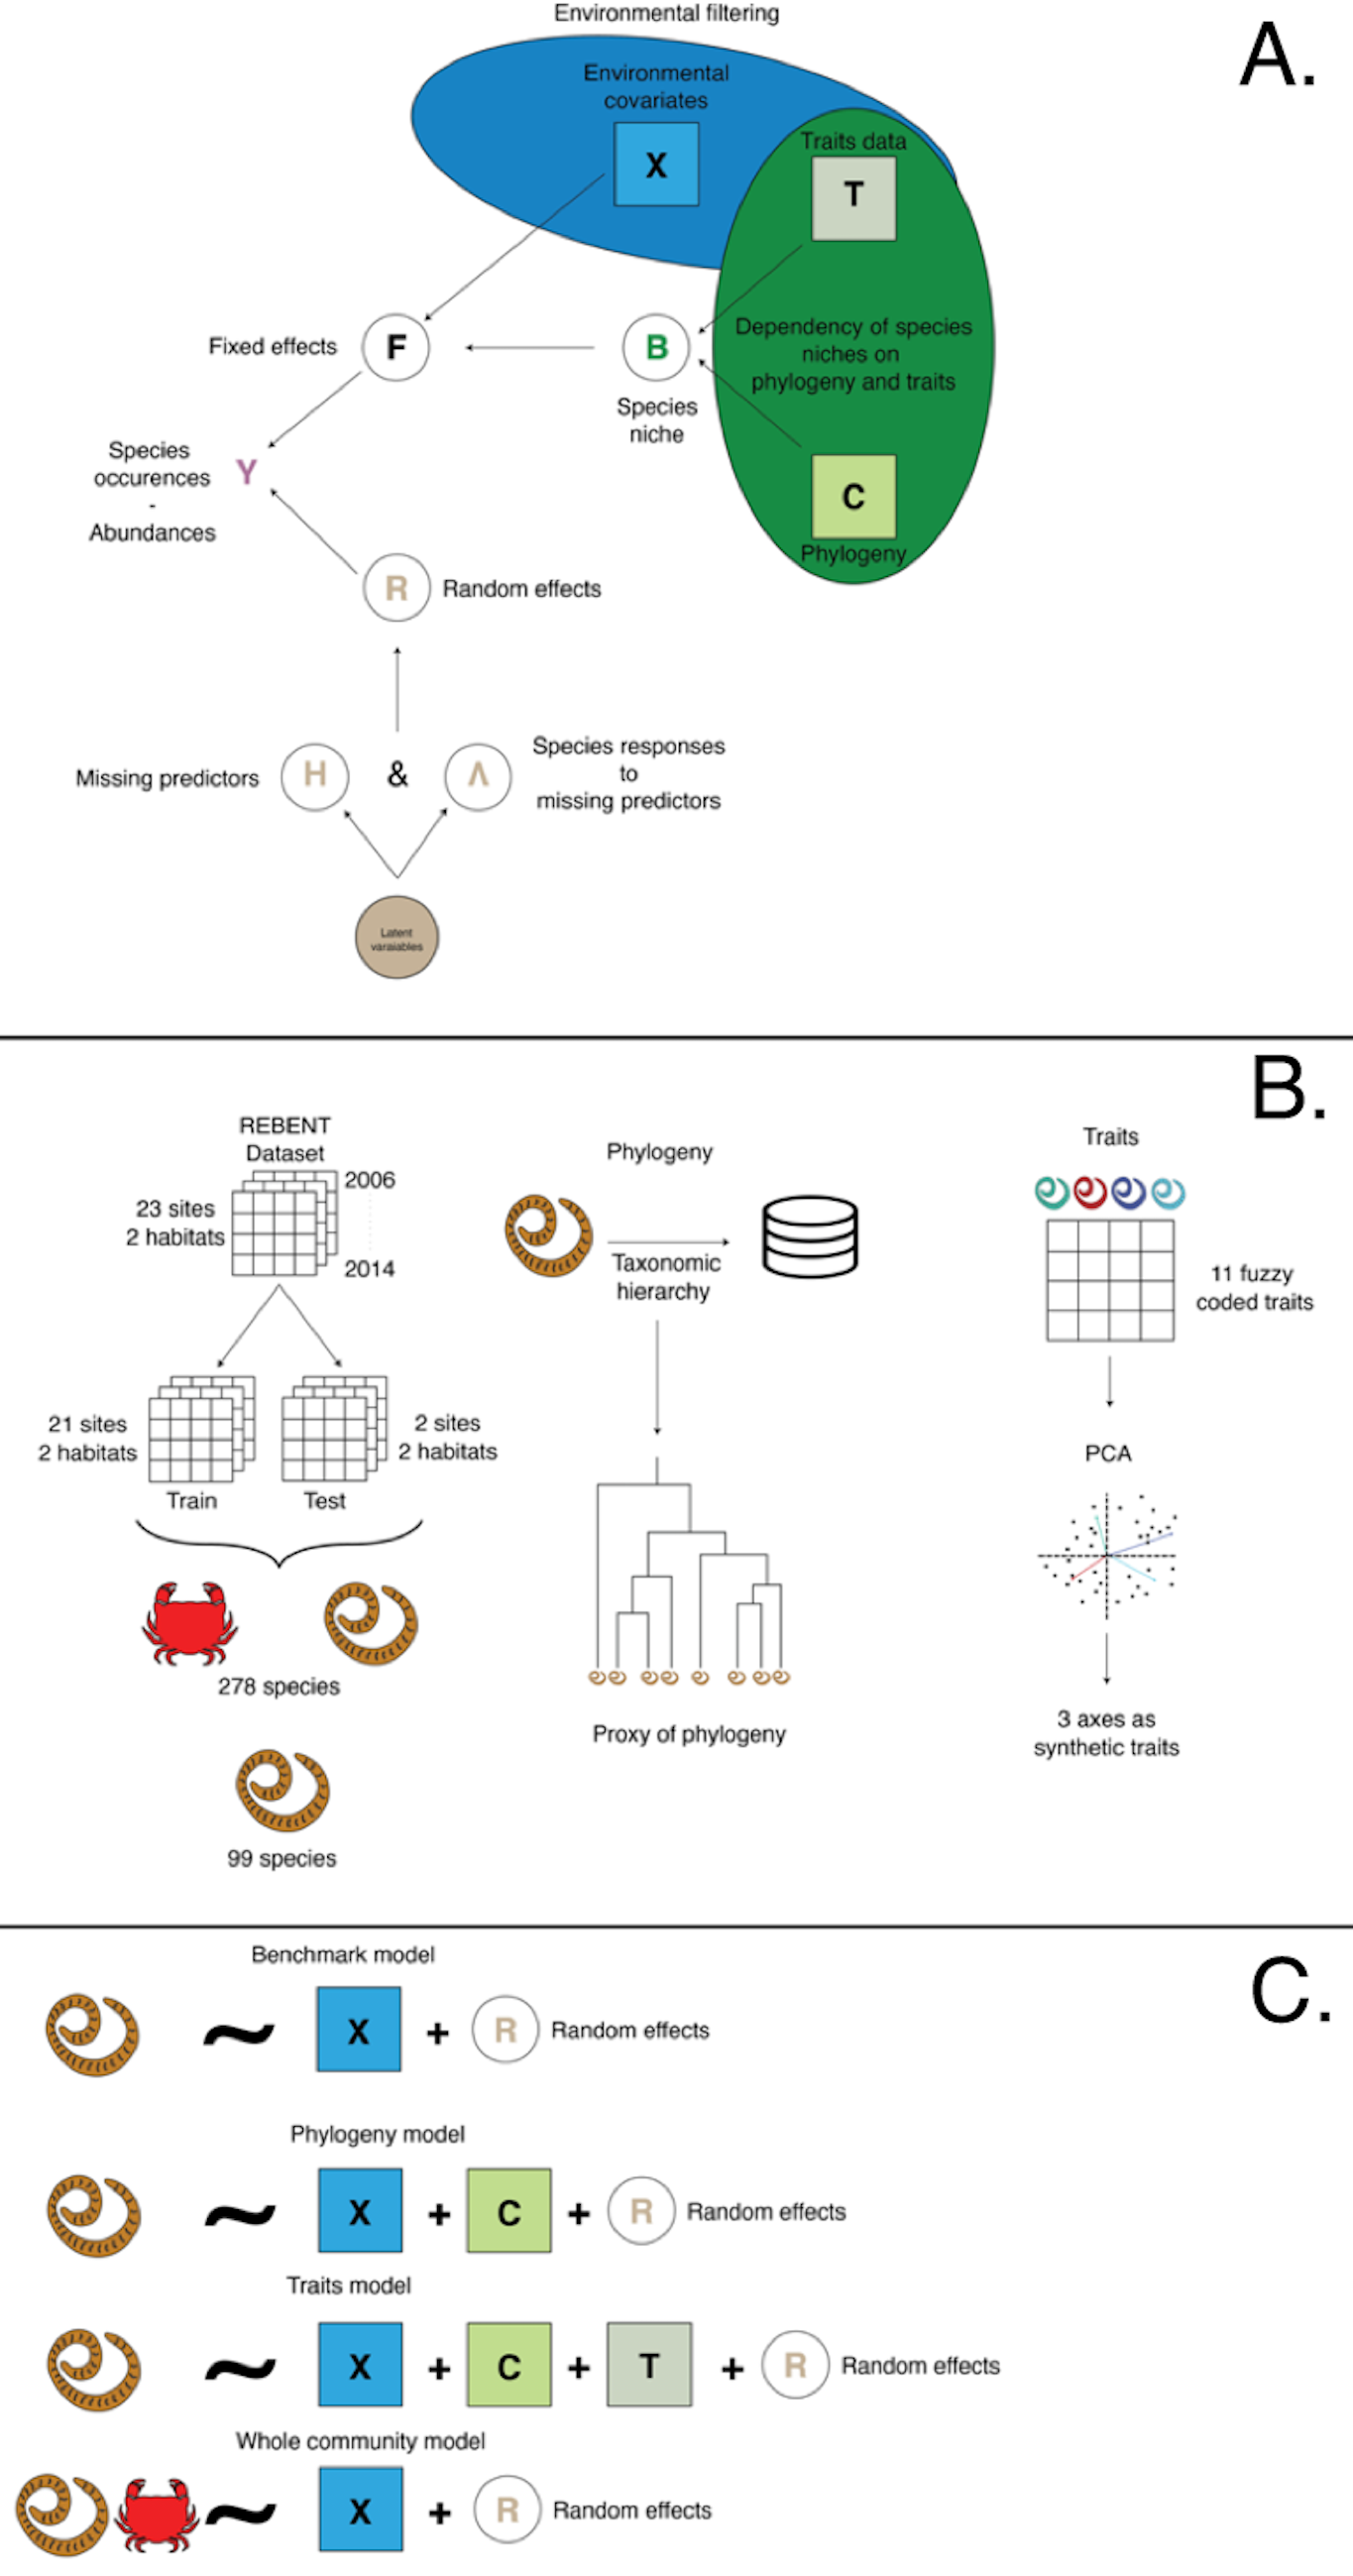
\includegraphics{figures/fig1.png}
\caption{Workflow of the study. A. Structure of a Hierarchical Model of
Species Community (HMSC) including environmental variables, phylogeny
and species-specific functional traits. B. Data pre-processing:
community data partitioning between train and test datasets, estimating
of phylogenetic distance between species (using taxonomic
classification) and dimension reduction of species-trait matrix using a
fuzzy-PCA. C. Summary of the four alternative model structures fitted
both on presence/absence and abundance data: the Benchmark, Phylogeny
and Traits \& Phylogeny models only considered polychaete species
assemblage data, while the Whole Community model includes information
related to additional species sampled alongside the target assemblage
(i.e.~non-target species that are not of direct interest but potentially
interact with the target assemblage). Random effects accounting for the
sampling year, site and habitat were included in all
models.}\label{fig:workflow}
}
\end{figure}

\hypertarget{hierarchical-modelling-of-species-community-hmsc}{%
\subsection{Hierarchical Modelling of Species Community
(HMSC)}\label{hierarchical-modelling-of-species-community-hmsc}}

``HMSC is a multivariate hierarchical generalised linear mixed model
adjusted with Bayesian inference rooted in assembly theory''
(\protect\hyperlink{ref-Ovaskainen_2020}{Ovaskainen \& Abrego 2020}). A
HMSC model is composed of two parts: one taking into account fixed
effects and the other taking into account random effects. The fixed part
models the realised niche (i.e., the set of environmental conditions
that is biotically suitable and accessible to the species; Ovaskainen \&
Abrego (\protect\hyperlink{ref-Ovaskainen_2020}{2020})) of each species
(B matrix), where each dimension of the niche is a covariate
(e.g.~temperature) included in the model (\cref{fig:workflow} ;
Ovaskainen \& Abrego (\protect\hyperlink{ref-Ovaskainen_2020}{2020})).
Including trait data enables estimating of species-specific expected
niche value by accounting for trait-environment relationships, where
species with similar traits are expected to respond similarly along
environmental gradients (\cref{fig:workflow} ; Ovaskainen \emph{et al.}
(\protect\hyperlink{ref-Ovaskainen_2017a}{2017b}) ; Ovaskainen \& Abrego
(\protect\hyperlink{ref-Ovaskainen_2020}{2020})). It is well-established
that phylogenetically-close species tend to share similar trait values
or niches (\protect\hyperlink{ref-Wiens_2010}{Wiens \emph{et al.}
2010}). Adding phylogenetic data to a HMSC model already including
traits is not necessarily redundant because it could capture residual
ecological information not included in the available trait data. This
can theoretically improve species niche estimates
(\protect\hyperlink{ref-Ovaskainen_2020}{Ovaskainen \& Abrego 2020}).
Inclusion of such additional pieces of information can moreover improve
model fit for rare species by borrowing information on traits- (or
phylogenetic-) environment relationships estimated for common species
that are similar in terms of traits (or phylogenetic; Ovaskainen \&
Abrego (\protect\hyperlink{ref-Ovaskainen_2020}{2020})). This property
is a main advantage of hierarchical models
(\protect\hyperlink{ref-Gelman_2020}{Gelman \emph{et al.} 2020}).

The random part of HMSC relies on latent variables. Specifically, for
each random effect, two matrices of latent variables are estimated
(\protect\hyperlink{ref-Ovaskainen_2017a}{Ovaskainen \emph{et al.}
2017b} ; \protect\hyperlink{ref-Tikhonov_2019b}{Tikhonov \emph{et al.}
2019} ; \protect\hyperlink{ref-Ovaskainen_2020}{Ovaskainen \& Abrego
2020}): the \(\Eta\) matrix (called site loadings) contains the values
of missing covariates not included in the model (\cref{fig:workflow} ;
Ovaskainen \emph{et al.}
(\protect\hyperlink{ref-Ovaskainen_2017a}{2017b}) ; Ovaskainen \& Abrego
(\protect\hyperlink{ref-Ovaskainen_2020}{2020})); while the \(\Lambda\)
matrix (called species loadings) corresponds to the response of the
species to missing covariates (\cref{fig:workflow} ; Ovaskainen \emph{et
al.} (\protect\hyperlink{ref-Ovaskainen_2017a}{2017b}) ; Ovaskainen \&
Abrego (\protect\hyperlink{ref-Ovaskainen_2020}{2020})). These
covariates thus capture residual variance, which can be due to various
factors including missing environmental features or the effect of biotic
interactions (\protect\hyperlink{ref-Ovaskainen_2017b}{Ovaskainen
\emph{et al.} 2017a} ;
\protect\hyperlink{ref-Ovaskainen_2017a}{Ovaskainen \emph{et al.} 2017b}
; \protect\hyperlink{ref-Ovaskainen_2020}{Ovaskainen \& Abrego 2020}).

\hypertarget{datasets}{%
\subsection{Datasets}\label{datasets}}

\hypertarget{faunistic-data}{%
\subsubsection{Faunistic data}\label{faunistic-data}}

Faunistic data come from the REBENT programme
(\href{https://rebent.ifremer.fr}{rebent.ifremer.fr}), which is a
station-based ongoing monitoring network initiated in 2003 to detect,
characterise and explain changes of coastal benthic macrofauna across
Brittany's coastline (Western France). Here, we focused on benthic
infaunal communities found in two soft-bottom habitats: intertidal bare
sediments and intertidal seagrass meadows (\emph{Zostera marina}). Data
from Boyé \emph{et al.} (\protect\hyperlink{ref-Boye_2019a}{2019}),
covering 23 sites (Fig. S1) monitored using the same protocol between
2006 and 2014, were used in this study. At each site, sampling consists
in the collection of three sediment cores of 0.03m\(^2\) that are pooled
together and considered as a single sampling unit at each site. For each
sampling event, individuals were identified to the lowest taxonomic
level possible (mostly species level; for simplicity we hereafter use
the term ``species''). A detailed description of the sampling
methodology is provided in (\protect\hyperlink{ref-Boye_2017}{Boyé
\emph{et al.} 2017} ; \protect\hyperlink{ref-Boye_2019a}{Boyé \emph{et
al.} 2019}). Overall, across a total of 375 sampling units (i.e.~unique
combination of years, sites and habitats), 861,997 individuals belonging
to 821 species were collected and identified.

\hypertarget{functional-traits-and-phylogeny-data}{%
\subsubsection{Functional traits and phylogeny
data}\label{functional-traits-and-phylogeny-data}}

We collated species-specific information related to functional traits
and phylogeny for inclusion in different models. These data were
particularly well resolved for the polychaete community which therefore
constitutes the main object of inference. Polychaeta is a taxonomic
group composed of numerous species exhibiting diverse lifestyles
(\protect\hyperlink{ref-Jumars_2015}{Jumars \emph{et al.} 2015}) that
can be used to monitor the health of benthic habitats
(\protect\hyperlink{ref-Giangrande_2005}{Giangrande \emph{et al.}
2005}). The polychaete traits data, which was available for the 99
polychaete species present in the training set, includes 11 fuzzy-coded
traits for a total of 41 modalities
(\protect\hyperlink{ref-Boye_2019a}{Boyé \emph{et al.} 2019}). Prior to
jSDM fitting, the dimensionality of the trait matrix was reduced using a
fuzzy-PCA with the \emph{fpca} function from the \emph{ade4} R package
(\protect\hyperlink{ref-Thioulouse_2018}{Thioulouse \emph{et al.}
2018}). The first three axes, which account for 59\% of the total
variance of the trait matrix, were included in the model as synthetic
traits data (\cref{fig:workflow}). The first axis distinguishes mobile
predatory species from sessile microphages; the second axis
differentiates semelparous species from iteroparous species; and, the
third axis separates burrowers from tube-dwellers (Fig. S5).

In complement to the traits information available for the 99 polychaete
species of interest, we retrieved their taxonomic classification through
the WoRMS database
(\href{https://www.marinespecies.org}{www.marinespecies.org}; assessed
in january 2020) and used this information as a proxy for phylogenetic
relationships (\cref{fig:workflow} ; Ricotta \emph{et al.}
(\protect\hyperlink{ref-Ricotta_2012}{2012}) ; Ovaskainen \& Abrego
(\protect\hyperlink{ref-Ovaskainen_2020}{2020})). Phylogenetic distances
between polychaete species were then estimated using the \emph{ape} R
package (\protect\hyperlink{ref-Paradis_2019}{Paradis \& Schliep 2019}).

\hypertarget{environmental-data}{%
\subsubsection{Environmental data}\label{environmental-data}}

Following Boyé \emph{et al.} (\protect\hyperlink{ref-Boye_2019a}{2019}),
we selected seven environmental variables to characterise the ecological
niche of each species within the target community. These seven variables
quantify different components of coastal environmental variability
including hydrology (sea water temperature, salinity and current
velocity), sedimentology (mud and organic matter content), substrate
heterogeneity (Trask index) and local wave exposure (fetch). For each of
these seven variables, the first and second degree polynomials were
computed to account for non-linear responses.

\hypertarget{comparison-of-alternative-model-structures}{%
\subsection{Comparison of alternative model
structures}\label{comparison-of-alternative-model-structures}}

The first model (benchmark model abbreviated as ``Bench'') only relies
on polychaete community data and environmental covariates
(\cref{fig:workflow}). The second model (phylogenetic model abbreviated
as ``Ph'') adds phylogenetic data to the Bench model
(\cref{fig:workflow}), which implies that rare species can thus benefit
from phylogenetic-environment relationships estimated for closely
related species (\protect\hyperlink{ref-Ives_2011}{Ives \& Helmus
2011}). The third model (traits \& phylogeny model abbreviated as
``TrPh'') adds traits data to the Ph model (\cref{fig:workflow}), which
means that rare species can benefit from traits-environment
relationships estimated for species presenting similar functional traits
(whereas phylogeny can capture ecological similarities between species,
which are not captured by trait similarity; Pollock \emph{et al.}
(\protect\hyperlink{ref-Pollock_2012}{2012})). Finally, the fourth model
(whole community model abbreviated as ``WhC''), adds information about
the whole community (i.e.~including non-polychaete species for a total
of 278 species) to the Bench model (only 99 polychaete;
\cref{fig:workflow}). This model does not include trait or phylogenetic
data for the sake of computation time. Each of these four models were
fitted twice, either using presence/absence or abundance data. All
models include the same random effects (\cref{fig:workflow}): a temporal
random effect to account for variability across years, a spatial random
effect to account for variability across sites and another spatial
random effect to account for variability across habitats (bare vs
seagrass).

\hypertarget{model-fitting-and-performance}{%
\subsection{Model fitting and
performance}\label{model-fitting-and-performance}}

\hypertarget{model-fitting-using-markov-chain-monte-carlo}{%
\subsubsection{Model fitting using Markov Chain Monte
Carlo}\label{model-fitting-using-markov-chain-monte-carlo}}

HMSC uses a Bayesian framework for model fitting where the posterior
distribution is sampled using a MCMC algorithm. For each model we ran 15
chains, each with 30,000 iterations. The first 10,000 iterations were
discarded as burn-in while the remaining were thinned every 20
iterations yielding 1,000 posterior samples per chain. Hence, in total,
15,000 posterior samples were recorded for each parameter. Model
convergence for each model parameter was assessed using the potential
scale reduction factor (\protect\hyperlink{ref-Gelman_1992}{Gelman \&
Rubin 1992}).

\hypertarget{assessing-model-performance-and-interpretability}{%
\subsubsection{Assessing model performance and
interpretability}\label{assessing-model-performance-and-interpretability}}

In order to independently assess models' predictive performance, we
splitted the dataset into a train and a test set. The training dataset
includes 180 sampling units defined as unique combinations of years
(varies between six and nine depending on sites), sites (21) and two
habitats (Fig. S1). From this dataset, that originally contained 519
species, we removed the species that occurred less than four times
across the 180 observational units to avoid convergence issues and poor
model inference, leading to the removal of 241 species. The remaining
278 species encompassed the 99 polychaete species that made up the
target community and the 142 non-target species that were included in
the WhC model. The test dataset was composed of 35 sampling units
related to all surveys over a 9-year period at two specific sites ,
where both habitats (i.e.~seagrass and bare sand) occur. Beyond the
presence of both habitats, these two sites were also chosen because they
occur in environmental conditions that can be considered average at the
scale of the region (thereby limiting extrapolation of the model; Boyé
\emph{et al.} (\protect\hyperlink{ref-Boye_2017}{2017}) ; Boyé \emph{et
al.} (\protect\hyperlink{ref-Boye_2022}{2022}) ; Toumi Chirine
(\protect\hyperlink{ref-Toumi_nd}{n.d.})) while still harbouring
different communities, representative of the known diversity gradient
across the region (\protect\hyperlink{ref-Boye_2017}{Boyé \emph{et al.}
2017} ; \protect\hyperlink{ref-Toumi_nd}{Toumi Chirine n.d.}).

To investigate jSDM's performance, models were evaluated using a set of
complementary metrics to evaluate both their explanatory (predictions
compared to observations of the train dataset) and predictive
(predictions compared to observations of the test dataset) powers
(\protect\hyperlink{ref-Wilkinson_2020}{Wilkinson \emph{et al.} 2020}).
To assess models' performance, both overall (i.e., across all species)
and at individual species level, we used AUC and root mean squared
errors (RMSE) for presence/absence and abundance models, respectively.
For the ``whole community'' model that most improved predictive power
(see results), we further explored species-specific gain in explanatory
power by examining potential correlations between (i) RMSE and the
proportion of presences and (ii) RMSE and average abundance using the
Kendall rank correlation coefficient.

While the AUC and the RMSE provide estimates of model performance,
either overall or for individual species, these measures only partially
capture model accuracy (or performance) at the community scale. Hence,
we also explored differences between observed and predicted community
composition (both for the train and test datasets) by decomposing the
total beta diversity (using the Sørensen index) into species turnover
and nestedness using the \emph{betapart.temp} function from the
\emph{betapart} R package (\protect\hyperlink{ref-Baselga_2010}{Baselga
2010} ; \protect\hyperlink{ref-Baselga_2022}{Baselga \emph{et al.}
2022}). For abundance models, predictions were transformed to
presence/absence before computing beta diversity (i.e.~all non-zero
abundance predictions were considered as presences). Thus, this
framework assigns a total beta diversity of zero to a model predicting
the exact observed community, whereas a model predicting a completely
different community compared to observations is associated with a total
beta diversity of one. Moreover, using Baselga \emph{et al.} (2022)'s
framework, we decomposed beta diversity (i.e.~predicted error in
community composition) according to two components: (1) turnover, if
model correctly estimates observed species richness but mispredicts
species identity and (2) nestedness, if model correctly predicts the
identity of observed species but omits some.

To assess model interpretability, we calculated the proportion of
explained variance attributed either to environmental covariates (fixed
effects) or to random effects. To evaluate the effect of model structure
on estimated species-environment relationships, we classified the shapes
of estimated response curves inferred from the different models
according to nine categories that characterise both their direction
(decline, null or increase) and their acceleration (decelerated,
constant or accelerated) (\protect\hyperlink{ref-Rigal_2020}{Rigal
\emph{et al.} 2020}). We then looked for differences between models in
terms of proportion of estimated response curves across each of these
nine categories. Finally, to compare changes in random effects across
models, we estimated differences between the Bench model and the best
performing model in terms of residual co-occurrence patterns. We
specifically quantified differences between models in both magnitude and
sign of residual species-species correlations using the following index:

\[\text{Index} = |corr_{\text{best model}} - corr_{\text{benchmark}}| \times sign(corr_{\text{best model}} \times corr_{\text{benchmark}})\]

\hypertarget{results}{%
\section{Results}\label{results}}

Both MCMC convergence and effective sample size of the different jSDMs
were satisfactory (see Appendix B).

\hypertarget{model-fit-predictive-power}{%
\subsection{Model Fit \& Predictive
power}\label{model-fit-predictive-power}}

\hypertarget{species-level}{%
\subsubsection{Species level}\label{species-level}}

Presence/absence models presented an excellent explanatory power as
reflected by mean AUC estimates greater than 0.9 (Fig. S4). Conversely,
their predictive power was rather low given a mean AUC estimate of
\textasciitilde0.65 (Fig. S4). For abundance models, mean RMSE computed
on the training set ranged from 8.94 to 9.35 (Fig. S4). Their predictive
power was heterogeneous with the whole community (WhC) model presenting
the highest performance (\(\text{mean RMSE} = 5.83\)) followed by the
benchmark model (Bench) (\(\text{mean RMSE} = 53.7\)), the phyloheny
(Ph) model (\(\text{mean RMSE}=63.7\)) and the traits \& phylogeny model
(\(\text{mean RMSE} = 95.3\)) (Fig. S4).

Relative to the benchmark model (\cref{fig:fig2}), model explanatory
power only sightly decreased for both TrPh (mean increase in RMSE +0.8\%
and decrease in AUC of -0.6\%) and Ph models (mean increase in RMSE of
+0.5\% and decrease in AUC -0.6\%). Explanatory power only slightly
increased for the WhC models (mean decrease in RMSE of -3.6\% and
increase in AUC +0.3\%). In terms of predictive power, performance
mostly increased for the WhC abundance model with a mean decrease in
RMSE of 26\% relative to the benchmark model. This improvement concerned
62 species (mean decrease in RMSE of -49.3\%; 10h and 90th deciles
{[}-94.8\% ; -9.7\%{]} for these species) whereas 12 species presented a
performance decrease (+36\% RMSE; 10th and 90th deciles {[}10\% ;
70.1\%{]}). Only 32 and 36 species were improved for TrPH and Ph models,
with mean decrease/increase in RMSE of 26.5\% and 24.9\% across all
species, respectively.

Model explanatory performance increased for the most common (correlation
between RMSE and proportion of presence: Kendall's τ = -0.28, p-value
\textless{} 1e-5) and abundant (correlation between RMSE and average
species abundance: Kendall's τ = -0.29, p-value \textless{} 1e-4).

\begin{figure}
\hypertarget{fig:fig2}{%
\centering
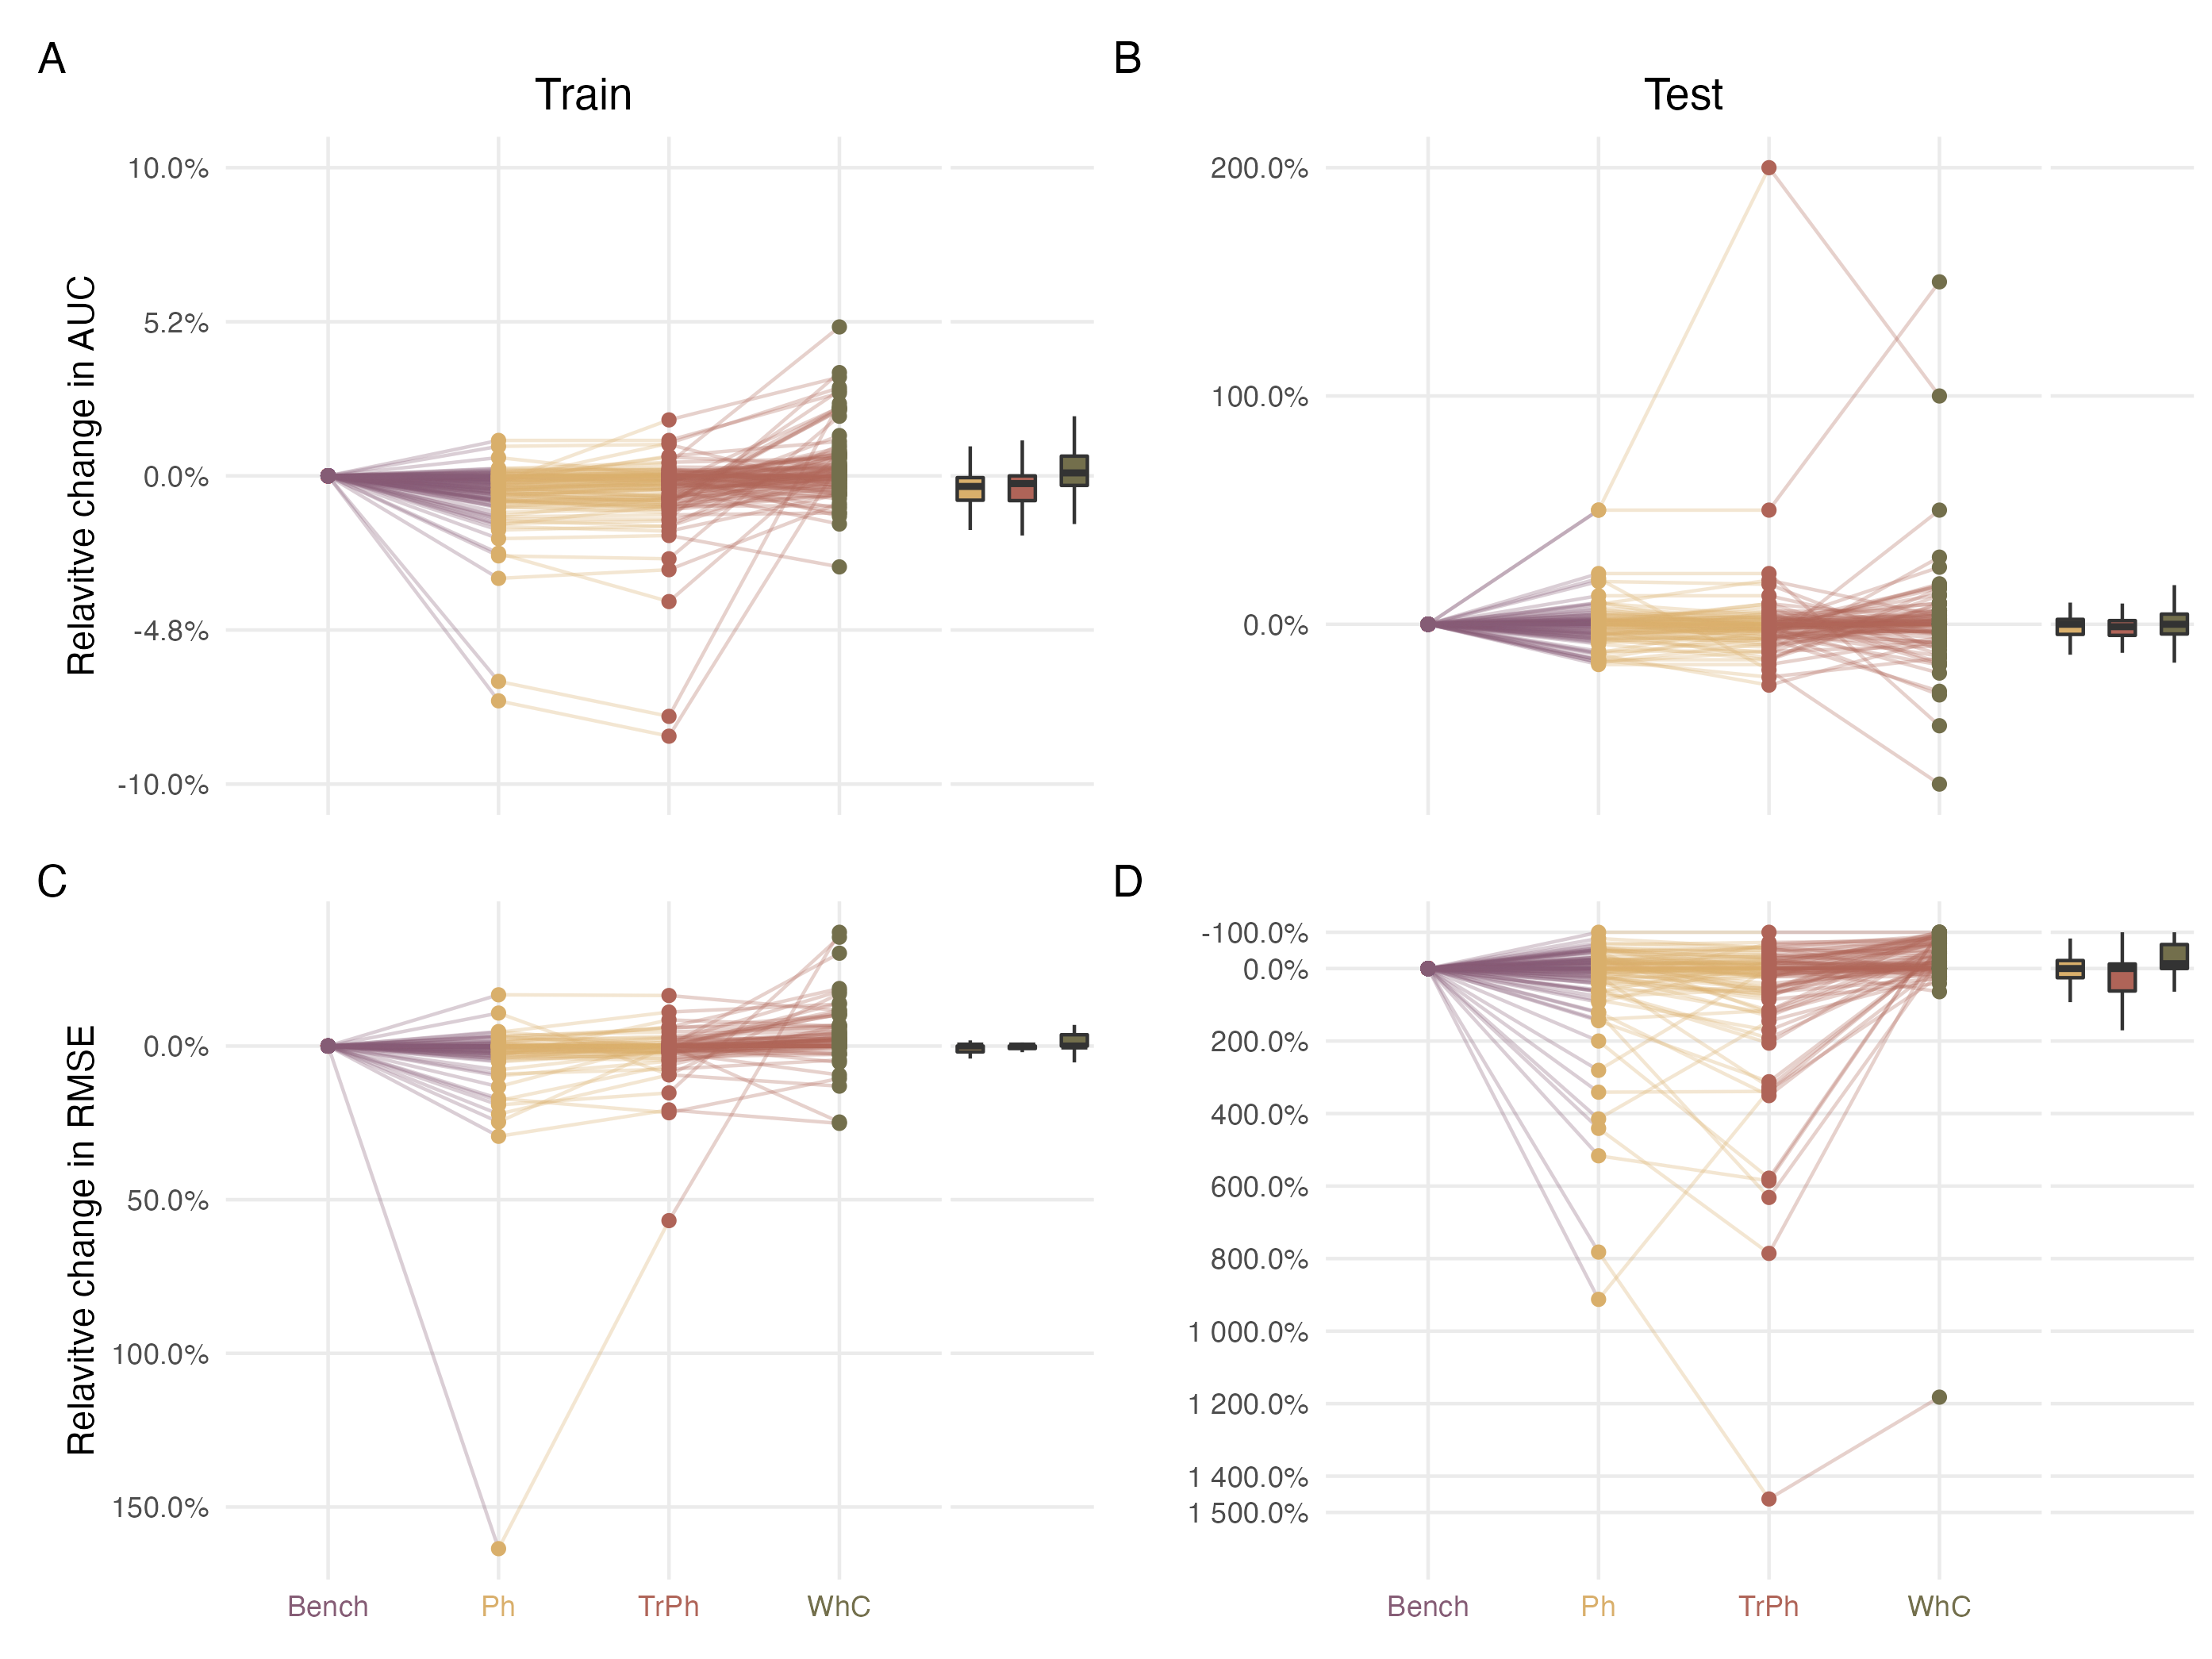
\includegraphics{figures/fig2.png}
\caption{Relative change in explanatory (left column; panels A and C)
and predictive (right column; panels B and D) power of different model
structures (as colour-coded: purple for benchmark (Bench), yellow for
phylogeny (Ph), red for traits \& phylogeny (TrPh), and green for whole
community (WhC) models). Relative changes (in \%) are expressed relative
to the benchmark fitted on presence/absence (top row; panels A and B) or
abundance (bottom row; panels C and D) data. In all panels, points above
the zero line (i.e.~increase in AUC for panels A-B but decrease in RMSE
for panels C-D) indicate performance gain.}\label{fig:fig2}
}
\end{figure}

\hypertarget{community-level}{%
\subsubsection{Community level}\label{community-level}}

On the training set, the median Sørensen dissimilarity index, which
ranged from 0.36 to 0.38 across all models (both presence/absence and
abundance), suggests that predicted communities are relatively similar
to observed communities (Fig. S8 and Fig. S9). Errors were equally
distributed between turnover and nestedness (Fig. S8 and Fig. S9).
However, relative to observed communities in the test data set,
abundance models predictions presented a median Sørensen dissimilarity
of 0.65 while dissimilarity reached 0.72 for presence/absence models
(Fig. S8 and Fig. S9). Greater dissimilarity between predicted and
observed communities in the test dataset relative to the training
dataset is a direct consequence of models' limited predictive power at
the species level (see above and Fig. S8 and Fig. S9). Note that
proportion of nestedness errors is greater in the WhC model than in
other models, suggesting that this model tends to correctly predict the
presence of a subset of the observed species assemblage composition
(Fig. S8 and Fig. S9).

\hypertarget{variance-partitioning}{%
\subsection{Variance partitioning}\label{variance-partitioning}}

The amount of variance explained by each model can be partitioned
between environmental covariates and random effects. For all models,
environmental variables account for most (more than 75\% ± 18\%, mean ±
s.d.) of the variance (Fig. S7). However, a larger part of variance is
explained by random effects in the WhC model compared to the Bench model
(Fig. S7). Relative to the Bench model, the median relative change in
variance explained by random effects increased by 8.6\% for the Ph
model, 19.9\% for the TrPh model and 35.4\% for the WhC model
(\cref{fig:fig3}). Similar results were obtained for presence/absence
models (\cref{fig:fig3}).

\begin{figure}
\hypertarget{fig:fig3}{%
\centering
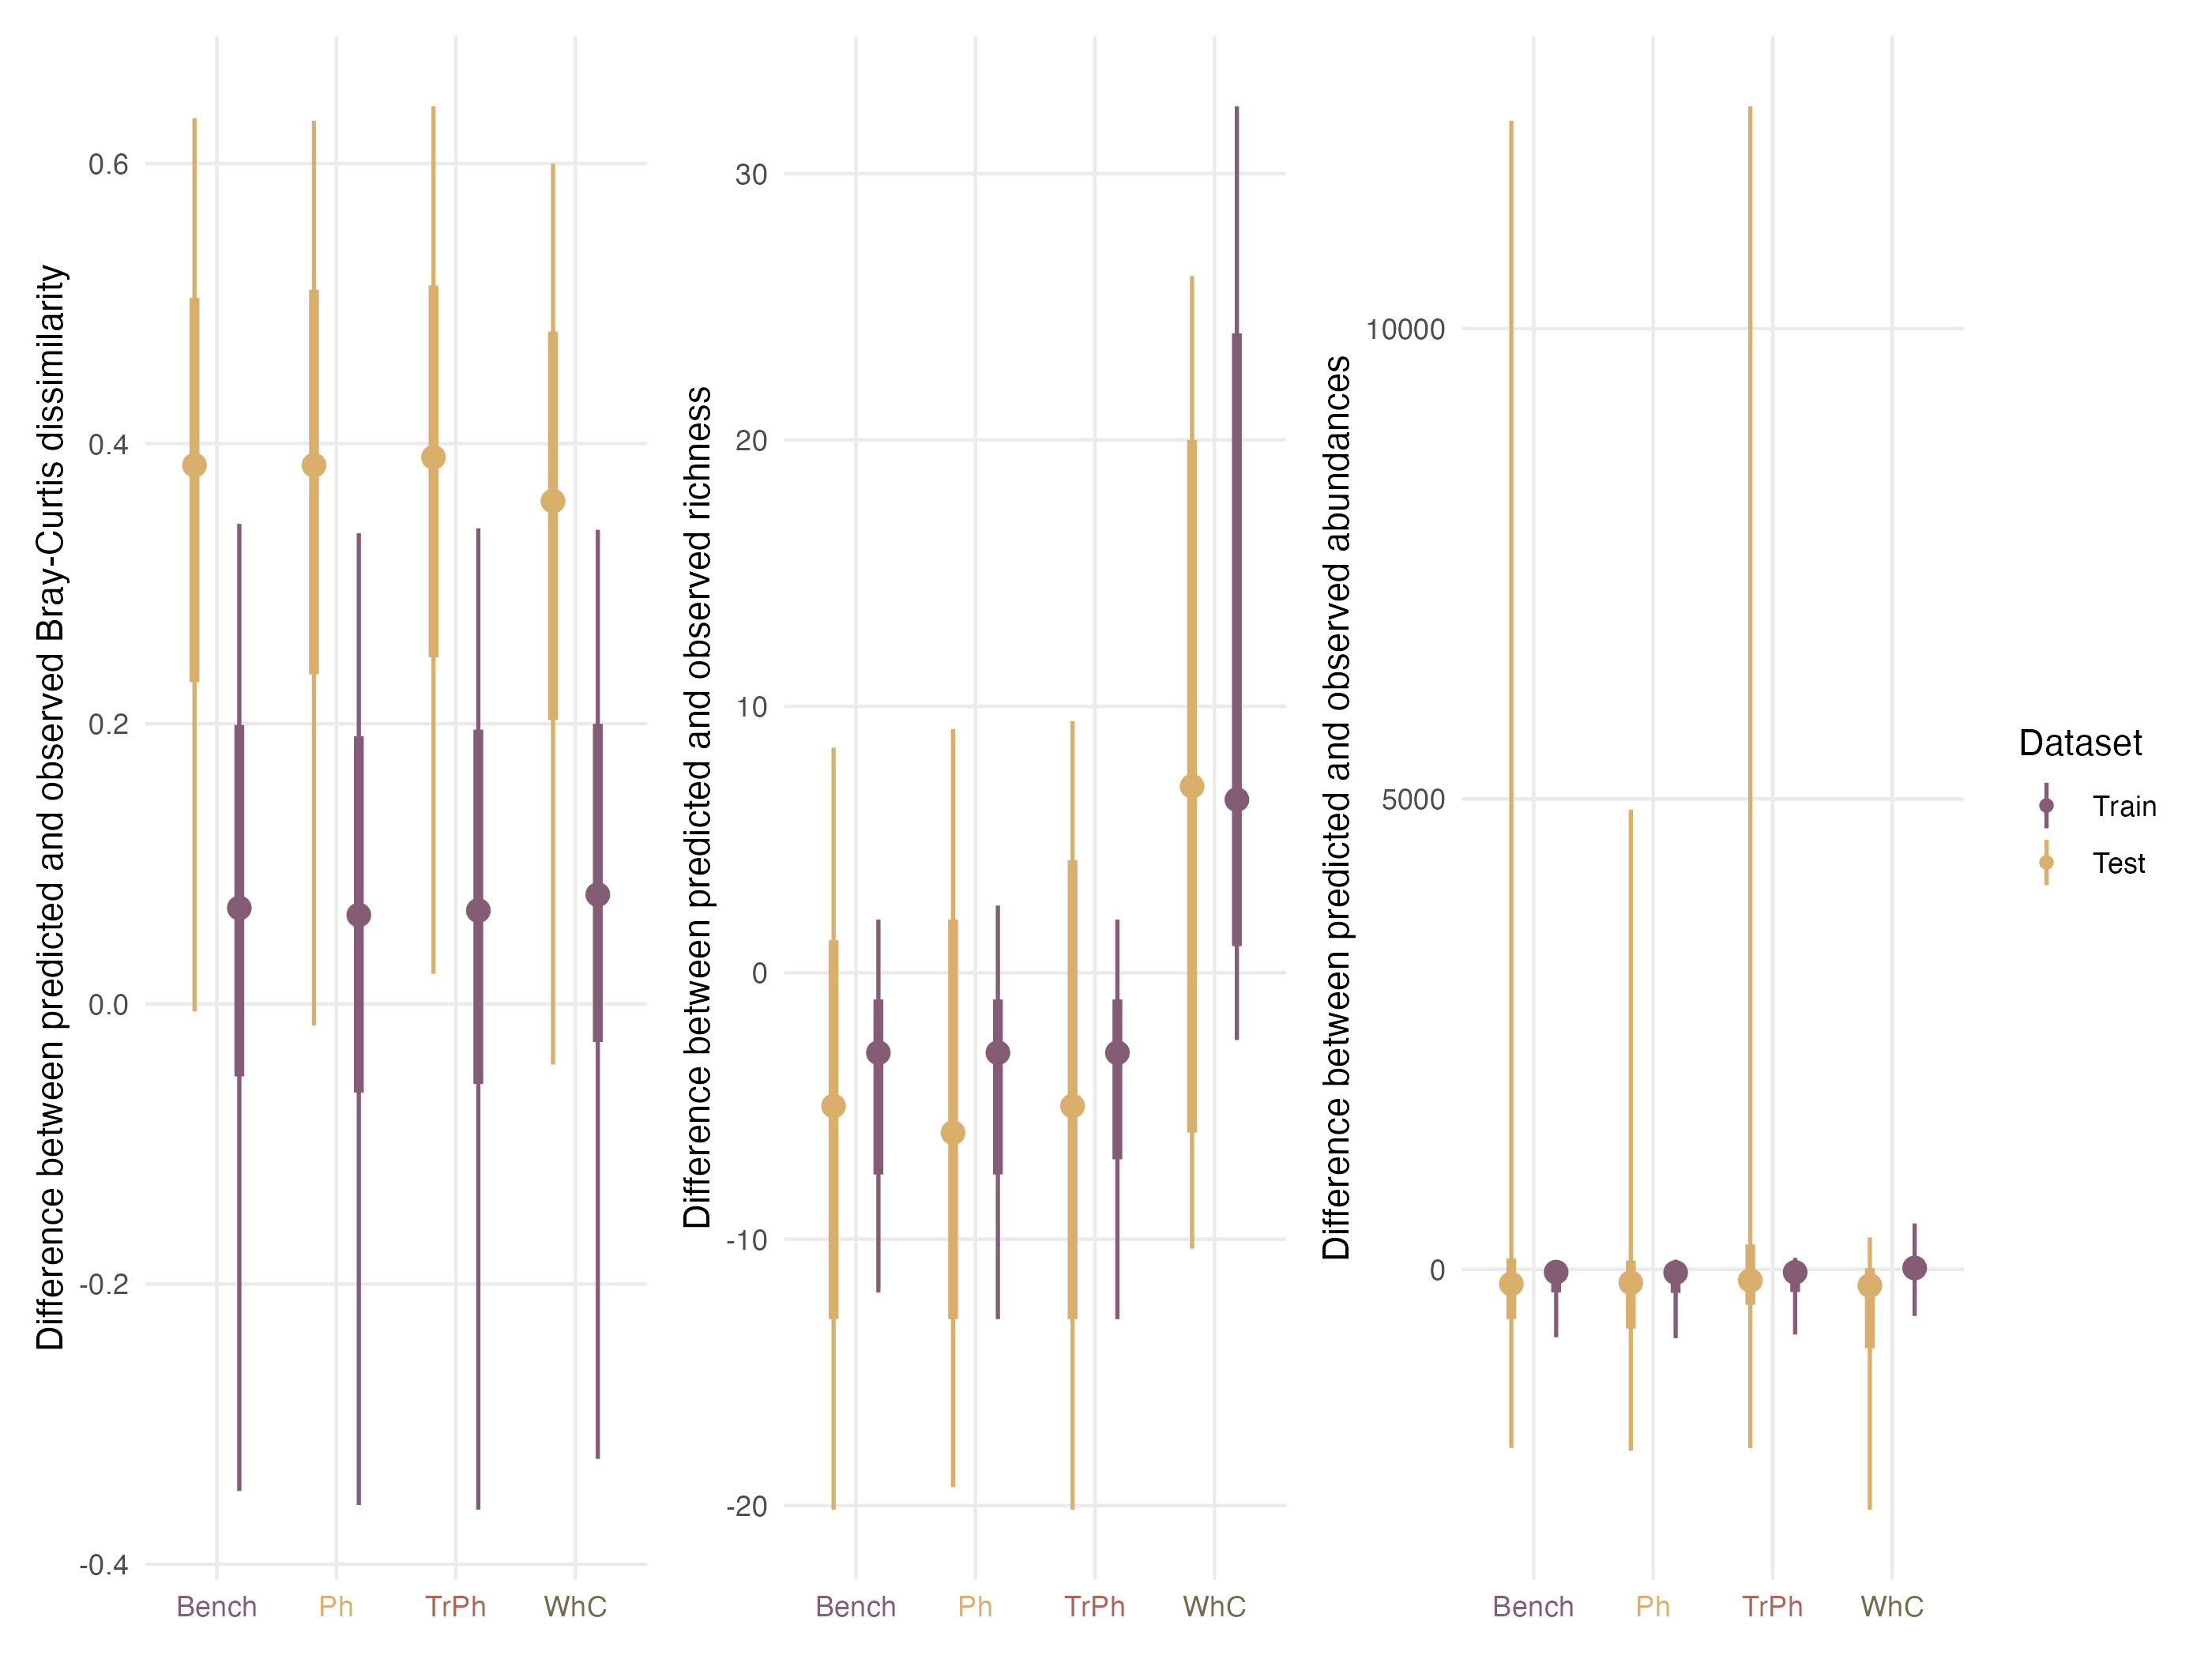
\includegraphics{figures/fig3.png}
\caption{Relative change in variance explained by environmental
predictors (left column) and by random effects (right column) according
to alternative models as colour-coded (purple for Benchmark (Bench),
yellow for phylogeny (Ph), red for traits \& phylogeny (TrPh), and green
for whole community (WhC) models). Percentage change is expressed
relative to the benchmark model fitted with presence/absence (top
panels) or abundance (bottom panels) data. In all panels, positive
(negative) values point to an increase (decrease) in the proportion of
variance explained by the focal model relative to the benchmark
model.}\label{fig:fig3}
}
\end{figure}

\hypertarget{species-niche-estimated}{%
\subsection{Species niche estimated}\label{species-niche-estimated}}

For all abundance models, more than 60\% of estimated response curves
were flat, suggesting a lack of ecologically meaningful
species-environment relationships (\cref{fig:fig4}). This proportion
even reached more than 80\% for the WhC model. Almost no convex or
concave responses curves were estimated for abundance models. Meaningful
species-environment relationships essentially included constant or
accelerated declines, which respectively represented \textasciitilde10\%
and \textasciitilde15\% of estimated response curves for the three
models that do not include the whole community (i.e.~Bench, TrPh and Ph)
(\cref{fig:fig4}). For the WhC model, these percentages dropped to
4.62\% and 9.24\%, respectively (\cref{fig:fig4}). Similar results were
obtained for presence/absence models (Fig. S10).

\begin{figure}
\hypertarget{fig:fig4}{%
\centering
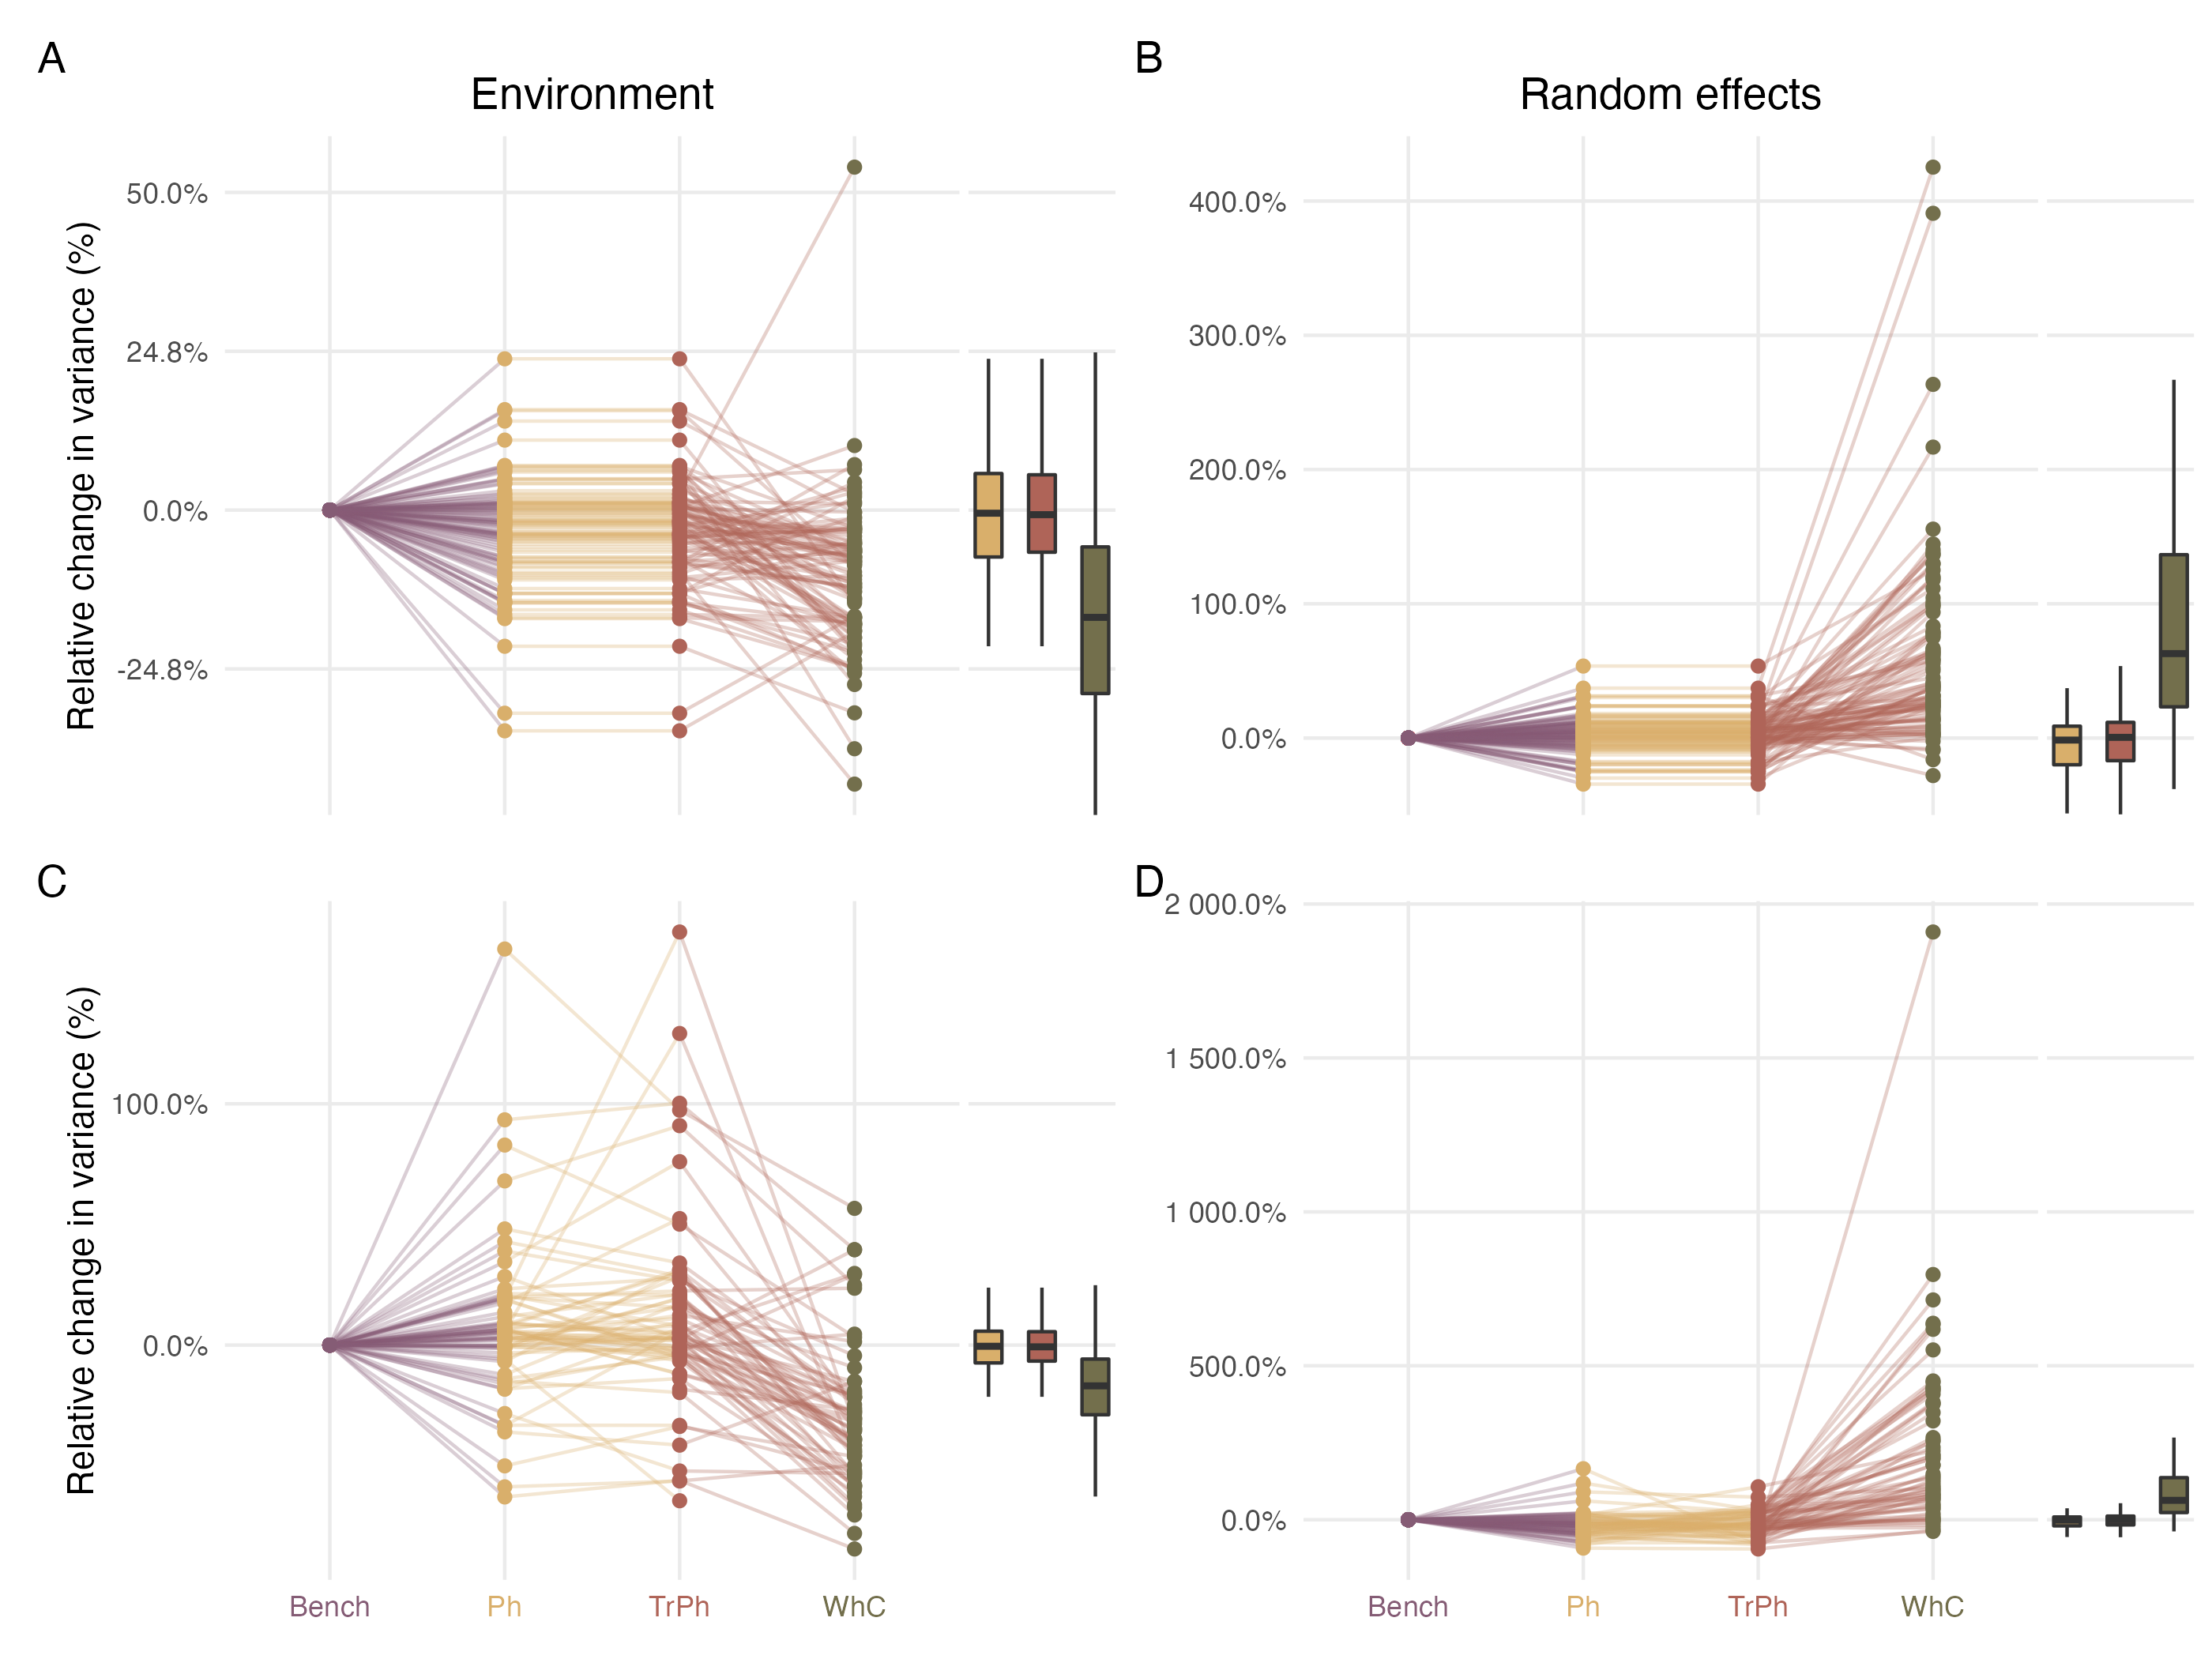
\includegraphics{figures/fig4.png}
\caption{Number (y-axis) and proportion (indicated above individual
bars) of response curves (i.e.~one for each species-predictor
combination) according to the nomenclature (nine shapes highlighted by
the black curve in each panel) defined by Rigal \emph{et al.}
(\protect\hyperlink{ref-Rigal_2020}{2020}) for different abundance model
structures. See Fig. S10 for a similar representation for
presence-absence models.}\label{fig:fig4}
}
\end{figure}

Both abundance- and presence/absence TrPh models (which include species
functional traits) reveal some meaningful trait-environment
relationships between the first fuzzy-PCA axis and the seven
environmental predictors. This suggests that the occurrence of certain
traits is likely favoured (or hindered) under certain environmental
conditions (Fig. S6). For instance, mobile predatory species were more
negatively affected by fetch than sessile suspensivores (Fig. S6).
Moreover, increase in organic matter concentration and decrease in
current velocities were associated with higher abundances of
suspensivore populations.

\hypertarget{exploring-the-residual-correlation}{%
\subsection{Exploring the residual
correlation}\label{exploring-the-residual-correlation}}

Since all models included the same random effects, residual correlation
matrices are comparable. Here, we compared residual correlations between
the Bench model and the WhC model both when fitted to presence/absence
or abundance data. We specifically considered the WhC model for this
specific comparison, because of (1) its higher performances relative to
alternative models and (2) the larger proportion of variance explained
by random effects in this model relative to others (\cref{fig:fig3}).

Residual correlations estimated by the WhC model were similar to those
estimated by the Bench model, regardless of whether the models were
fitted on presence/absence or abundance data (\cref{fig:fig5} and Fig.
S11). Yet, agreement between models varied across the different random
effects. For instance, when comparing residuals between Bench and WhC
fitted on abundance data, correlation was low for random site effects
(\(\text{R}^2 = 0.66\)), moderate for random habitat effects
(\(\text{R}^2 = 0.8\)) and high for random year effects
(\(\text{R}^2 = 0.91\)).

\begin{figure}
\hypertarget{fig:fig5}{%
\centering
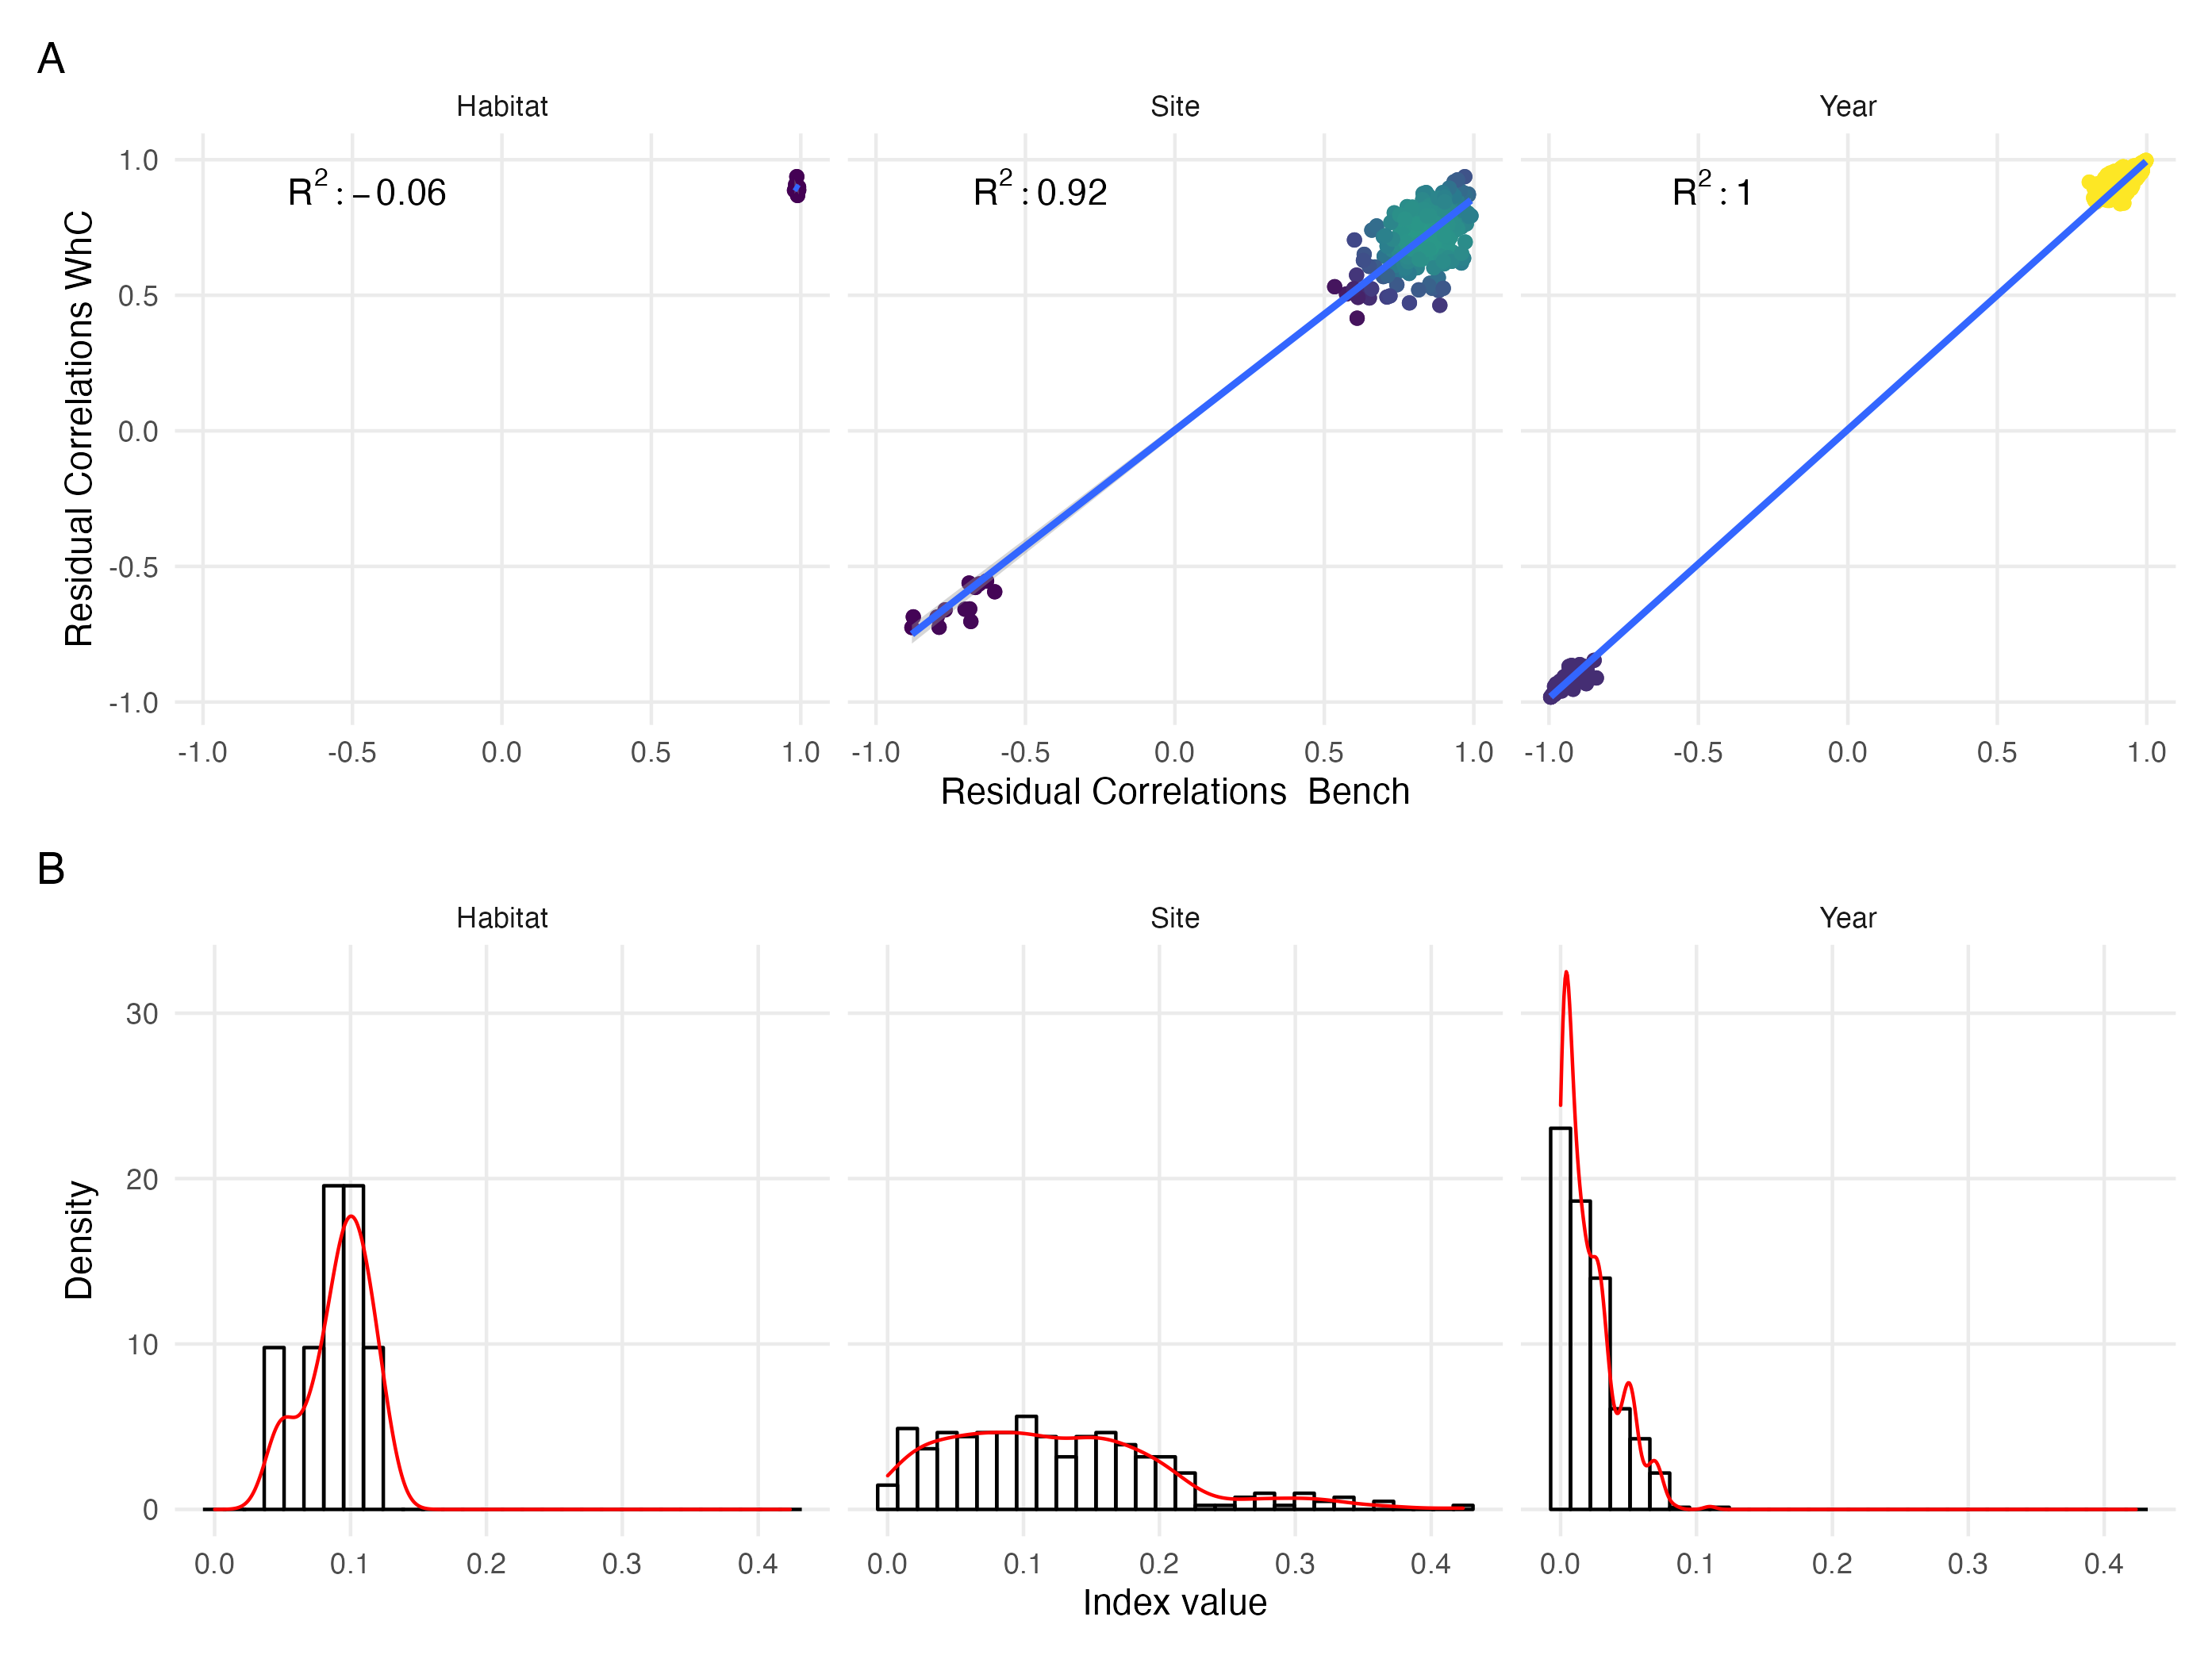
\includegraphics{figures/fig5.png}
\caption{(A) Comparison of residual correlations associated with the
three random effects estimated by the Whole Community Model (y-axis) and
the Benchmark model (x-axis) fitted on abundance data. The colour scale
highlights the density of points in each scatter plot. (B) Distribution
of the index measuring change in sign (sign change left to the zero
line, no change to the right) and magnitude (higher departure from the
zero line indicate higher difference) between residual correlations
estimated by the whole community model and the benchmark model adjusted
with abundance data for the three random effects (Habitat, Site,
Year).}\label{fig:fig5}
}
\end{figure}

The dedicated comparison index helps qualify how pairwise
species-species residual correlations change in sign and magnitude
between the Bench and the WhC models. For abundance- or presence/absence
models (\cref{fig:fig5} and Fig. S11), the index main modal
distribution, which is centred on zero, suggests an overall agreement
between residual correlations obtained from both models (\cref{fig:fig5}
and Fig. S11). While the right part of the distribution highlights
variation in the estimated magnitude of effect, on the left-hand part of
the distribution (negative values) indicates a sign inconsistency in
residual correlations between the two models. For abundance models, the
Habitat, Site and Year random effects are respectively associated with
13.3\%, 17.7\% and 6\% of sign inconsistencies in residual correlations
between the Bench model and the WhC model. Similar results were obtained
for presence/absence models.

\hypertarget{discussion}{%
\section{Discussion}\label{discussion}}

Case studies in community ecology typically rely on partial and
heterogeneous observations (\protect\hyperlink{ref-Pollock_2020}{Pollock
\emph{et al.} 2020}) but also on incomplete knowledge of target species
ecological features (e.g.~traits, phylogeny; Troudet \emph{et al.}
(\protect\hyperlink{ref-Troudet_2017}{2017})). In this paper we
investigated how jSDM performance varies depending on the type of
information included (i.e.~phylogeny, traits or data on non-target
species). While jSDMs have two main goals, i.e.~explaining and
predicting species distribution and community composition across space
and/or time (\protect\hyperlink{ref-Tredennick_2021}{Tredennick \emph{et
al.} 2021}), they have mostly been tested with regards to their
predictive power (\protect\hyperlink{ref-Norberg_2019}{Norberg \emph{et
al.} 2019}), and to some extent in terms of parameter estimates
(\protect\hyperlink{ref-Wilkinson_2020}{Wilkinson \emph{et al.} 2020}),
but only when fitted on presence/absence data
(\protect\hyperlink{ref-Norberg_2019}{Norberg \emph{et al.} 2019} ;
\protect\hyperlink{ref-Wilkinson_2020}{Wilkinson \emph{et al.} 2020}).
Yet, jSDMs are increasingly fitted on abundance data
(\protect\hyperlink{ref-Brimacombe_2020}{Brimacombe \emph{et al.} 2020})
and for explanatory purposes (\protect\hyperlink{ref-Abrego_2016}{Abrego
\emph{et al.} 2017} ; \protect\hyperlink{ref-Hakkila_2018}{Häkkilä
\emph{et al.} 2018}). Hence, there is a mismatch between current
understanding of jSDMs performance and their application by ecologists.
Here, we consolidate the assessment of jSDMs performance using
complementary metrics and evaluation methods. We characterise how
different aspects of model performances vary with changes in model
structure related to the type of information considered, which can
affect interpretability and conclusions drawn from these models.

We found that jSDM's performance, in particular predictive power of
abundance models, most increased when including information related to
the 179 non-target species sampled alongside with the 99 polychaete
species of interest. Given HMSC hierarchical structure
(\protect\hyperlink{ref-Poggiato_2021}{Poggiato \emph{et al.} 2021}),
inclusion of monitoring data related to other species likely improves
model performance for the target assemblage by capturing relevant
drivers that are not explicitly considered. For instance, inclusion of
monitoring data for other species can help describe target species'
realised niche by accounting for ecological processes related to
environmental conditions (including trait-mediated responses) or biotic
interactions that are not explicitly captured otherwise
(\protect\hyperlink{ref-Ovaskainen_2017a}{Ovaskainen \emph{et al.}
2017b}). In jSDMs, unquantified ecological processes can be estimated
using latent variables from model residual correlation matrix. While
this feature of jSDMs originally yielded the potential to capture biotic
interactions, it is now well-established that potential biotic signals
captured by jSDMs are largely confounded by other factors. These include
missing environmental variables
(\protect\hyperlink{ref-Dormann_2018}{Dormann \emph{et al.} 2018} ;
\protect\hyperlink{ref-Zurell_2018}{Zurell \emph{et al.} 2018} ;
\protect\hyperlink{ref-Blanchet_2020}{Blanchet \emph{et al.} 2020}),
scale mismatch between study organism responses and available
environmental variables (\protect\hyperlink{ref-Potter_2013}{Potter
\emph{et al.} 2013}), coarse spatial resolution of environmental
variables (\protect\hyperlink{ref-Zurell_2018}{Zurell \emph{et al.}
2018} ; \protect\hyperlink{ref-Konig_2021}{König \emph{et al.} 2021}).

Importantly, while including non-target species improved predictive
performance in our case study, benefits of accounting for non-target
species might vary depending on robustness of non-target species
monitoring data (e.g.~detection issues), their role within the ecosystem
(e.g.~engineer species are likely more influential on local communities
than rare transient species), or processes shaping the target assemblage
(if influence of abiotic factors dominates, then adding other species
will have marginal consequences on model performance). Furthermore, a
specific investigation would be required to determine the optimal number
of non-target species to include : for instance using simulated datasets
to overcome limitations related to real world datasets
(\protect\hyperlink{ref-DiRenzo_2022}{DiRenzo \emph{et al.} 2022}).
While species communities and assemblages are largely defined
arbitrarily (\protect\hyperlink{ref-Stroud_2015}{Stroud \emph{et al.}
2015}), A systematic assessment of jSDM performance as increasing number
of non-target species, across different functional or trophic roles
would be valuable to delineate which ecological units to include (or
not) to improve model performance for the species of
management/conservation interests.

In practice, ecological studies often focus on a certain guild or
taxonomic group (e.g.~fish, birds) given data collection (consistent
sampling methodology) or availability constraints (traits and/or
phylogeny biased toward some taxonomic groups, Tyler \emph{et al.}
(\protect\hyperlink{ref-Tyler_2012}{2012}) and usually centralised in
taxonomic-centred repositories {[}e.g.~FishBase; Froese \& Pauly
(\protect\hyperlink{ref-Froese_2022}{2022}){]}), rather than for
ecological reasons (e.g.~all potential interactions well captured by the
data at hand). In this study, dedicated focus on polychaetes was
primarily guided by data availability (species-traits matrices available
from Boyé \emph{et al.} (\protect\hyperlink{ref-Boye_2019a}{2019}) only
included polychaetes) rather than for ecological reasons, although the
fact that this taxonomic group is numerically dominant and highly
diverse in terms of lifestyles and functional roles
(\protect\hyperlink{ref-Jumars_2015}{Jumars \emph{et al.} 2015} ;
\protect\hyperlink{ref-Giangrande_1997}{Giangrande 1997}) was the reason
that originally motivated trait-data collection.

jSDMs have already been used to model the distribution of a wide variety
of species ranging from micro-organisms
(\protect\hyperlink{ref-Minard_2019}{Minard \emph{et al.} 2019} ;
\protect\hyperlink{ref-Pichler_2021}{Pichler \& Hartig 2021}) to
megafauna (\protect\hyperlink{ref-Rocha_2017}{Rocha \emph{et al.} 2017}
; \protect\hyperlink{ref-Brimacombe_2020}{Brimacombe \emph{et al.}
2020}) inhabiting many different ecosystems. Here, while we studied
communities associated with two specific coastal habitats, i.e.~seagrass
and sand, that have original characteristics as they are located at the
land-sea interface (\protect\hyperlink{ref-Boye_2019a}{Boyé \emph{et
al.} 2019}), our case study reflects typical aspects of applied
ecological research. These include issues related to data limitation and
availability but also typical features of ecological communities
(e.g.~prevalence of rare and transient species; Magurran \& Henderson
(\protect\hyperlink{ref-Magurran_2003}{2003}) ; Snell Taylor \emph{et
al.} (\protect\hyperlink{ref-SnellTaylor_2018}{2018})). Our results
provide some insights on trait-environment relationships but these
contributions of functional ecology in jSDMs are likely limited by trait
data quality and availability (\protect\hyperlink{ref-Tyler_2012}{Tyler
\emph{et al.} 2012} ; \protect\hyperlink{ref-deJuan_2022}{Juan \emph{et
al.} 2022}). For instance, we found an interaction between trophic
modalities (i.e.~microphagous versus macrophagous diet) and fetch (Fig.
S15), indicating that organisms that filter on small particles are less
likely to occur in wave-exposed sites where high levels of sediment
resuspension can block their filtering systems
(\protect\hyperlink{ref-Manning_2014}{Manning \emph{et al.} 2014}).
Conversely macrophagous organisms are less impacted by fetch. Yet, most
trait-environment relationships, and most species-environment
relationships were flat suggesting that polychaete assemblages are
driven by processes other than abiotic ones, including neutral processes
(\protect\hyperlink{ref-Boye_2019a}{Boyé \emph{et al.} 2019}). However,
the lack of contribution of other trait-environment relationships in our
model could also be related to a mismatch between trait data,
environmental data, and the ecological processes at play
(\protect\hyperlink{ref-deJuan_2022}{Juan \emph{et al.} 2022}). For
instance, the physical coastal environment is highly dynamic; a feature
that is only partially characterised by our environmental variables that
summarise average climatological conditions (but not extreme events or
annual/seasonal variability). Likewise, the list of available
fuzzy-coded traits only partially captures species capacity to adapt to
frequent disturbances or environmental variability
(\protect\hyperlink{ref-Violle_2012}{Violle \emph{et al.} 2012} ;
\protect\hyperlink{ref-deJuan_2022}{Juan \emph{et al.} 2022}). Most
ecological studies are likely to face similar trade-offs where the
potential benefit of including traits within jSDMs is balanced out by
the effort needed to collect relevant trait information when missing. In
our case, while including traits does not improve model predictive
power, it enhances our understanding of species responses along
environmental gradients. Hence, if the goal is not prediction but
inference (\protect\hyperlink{ref-Tredennick_2021}{Tredennick \emph{et
al.} 2021}), including traits and proxies of phylogeny can facilitate
model interpretation, providing that explanatory power does not decrease
(as in our case), and that additional model parameters do not make
computation time impractical.

While guidelines have been developed to characterise the performance of
jSDM fitted on presence-absence data
(\protect\hyperlink{ref-Wilkinson_2020}{Wilkinson \emph{et al.} 2020}),
it is only recently that the predictive power of abundance-based models
has been explored (\protect\hyperlink{ref-Waldock_2022}{Waldock \emph{et
al.} 2022}). Here, we used a set of complementary metrics to assess the
performance of both presence-absence and abundance models at the species
and community levels, the latter considering both alpha and beta
diversity. We also transposed a method initially developed for time
series (\protect\hyperlink{ref-Rigal_2020}{Rigal \emph{et al.} 2020}) to
provide an innovative way of characterising the response curves of each
species. Further, we bring together a set of approaches and propose a
new index to characterise and compare residual correlation matrices.
Overall, we provide a comprehensive framework for integrative assessment
and comparison of alternative jSDM performance.

Overall, our results provide new insights into the most appropriate
strategies for jSDM fitting, according to modelling objectives
(\protect\hyperlink{ref-Troudet_2017}{Troudet \emph{et al.} 2017}) and
available data. While the four models considered had similar explanatory
power, adding extra information to traditional jSDMs that only consider
abiotic predictors can prove useful in cases. For instance, adding
monitoring data for other non-target species can substantially increase
model predictive power by modifying inferred species-environment
relationships and residual correlation matrices. Similarly, adding
traits or phylogeny can improve model interpretability. Future studies
will be key to consolidate our findings on simulated case studies
(\protect\hyperlink{ref-Zurell_2010}{Zurell \emph{et al.} 2010} ;
\protect\hyperlink{ref-DiRenzo_2022}{DiRenzo \emph{et al.} 2022}), or
across contrasted ecosystems, for instance dominated either by
environmental filtering, or by competitive processes.

\hypertarget{author-contributions}{%
\subsection{Author Contributions}\label{author-contributions}}

MPM conceived the project with inputs from CV, AB, MC. CV analysed data
and led manuscript write-up. All authors had significant inputs to the
manuscript and approved this final version.

\hypertarget{acknowledgments}{%
\subsection{Acknowledgments}\label{acknowledgments}}

We are grateful to Marion Maguer and Vincent Le Garrec who conducted
fieldwork and laboratory analyses, as well as to supporting students and
staff involved in the REBENT monitoring programme coordinated by
Sandrine Derrien (MNHN) and its funding partners (Agence de l'eau
Loire-Bretagne, Région Bretagne, DREAL Bretagne). The authors would also
like to acknowledge the Pôle de Calcul et de Données Marines (PCDM) for
providing DATARMOR storage and computational resources.
\url{https://pcdm.ifremer.fr}. MPM is the recipient of an ANR early
career grant ANR-21-CE02-0006.

\hypertarget{references}{%
\section*{References}\label{references}}
\addcontentsline{toc}{section}{References}

\hypertarget{refs}{}
\begin{CSLReferences}{1}{0}
\leavevmode\vadjust pre{\hypertarget{ref-Abrego_2016}{}}%
Abrego, N., Dunson, D., Halme, P., Salcedo, I. \& Ovaskainen, O. (2017).
\href{https://doi.org/10.1111/oik.03674}{Wood-inhabiting fungi with
tight associations with other species have declined as a response to
forest management}. \emph{Oikos}, 126.

\leavevmode\vadjust pre{\hypertarget{ref-Baselga_2010}{}}%
Baselga, A. (2010).
\href{https://doi.org/10.1111/j.1466-8238.2009.00490.x}{Partitioning the
turnover and nestedness components of beta diversity}. \emph{Global
Ecology and Biogeography}, 19, 134--143.

\leavevmode\vadjust pre{\hypertarget{ref-Baselga_2022}{}}%
Baselga, A., Orme, D., Villeger, S., De Bortoli, J., Leprieur, F. \&
Logez, M. (2022).
\emph{\href{https://CRAN.R-project.org/package=betapart}{betapart:
Partitioning Beta Diversity into Turnover and Nestedness Components}}.

\leavevmode\vadjust pre{\hypertarget{ref-Blanchet_2020}{}}%
Blanchet, F.G., Cazelles, K. \& Gravel, D. (2020).
\href{https://doi.org/10.1111/ele.13525}{Co-occurrence is not evidence
of ecological interactions}. \emph{Ecology Letters}.

\leavevmode\vadjust pre{\hypertarget{ref-Boye_2022}{}}%
Boyé, A., Gauthier, O., Becheler, R., Le Garrec, V., Hily, C., Maguer,
M., \emph{et al.} (2022).
\href{https://doi.org/10.1111/1365-2745.13791}{Drivers and limits of
phenotypic responses in vulnerable seagrass populations: Zostera marina
in the intertidal}. \emph{Journal of Ecology}, 110, 144--161.

\leavevmode\vadjust pre{\hypertarget{ref-Boye_2017}{}}%
Boyé, A., Legendre, P., Grall, J. \& Gauthier, O. (2017).
\href{https://doi.org/10.1016/j.seares.2017.06.004}{Constancy despite
variability: Local and regional macrofaunal diversity in intertidal
seagrass beds}. \emph{Journal of Sea Research}, 130, 107--122.

\leavevmode\vadjust pre{\hypertarget{ref-Boye_2019a}{}}%
Boyé, A., Thiébaut, Éric, Grall, J., Legendre, P., Broudin, C., Houbin,
C., \emph{et al.} (2019).
\href{https://doi.org/10.1111/ddi.12987}{Trait-based approach to
monitoring marine benthic data along 500 km of coastline}.
\emph{Diversity and Distributions}, 25, 1879--1896.

\leavevmode\vadjust pre{\hypertarget{ref-Brimacombe_2020}{}}%
Brimacombe, C., Bodner, K. \& Fortin, M.-J. (2020).
\href{https://doi.org/10.1111/ecog.05452}{Inferred seasonal interaction
rewiring of a freshwater stream fish network}. \emph{Ecography}, n/a.

\leavevmode\vadjust pre{\hypertarget{ref-Brudvig_2022}{}}%
Brudvig, L.A. \& Catano, C.P. (2022).
\href{https://doi.org/10.1111/rec.13380}{Prediction and uncertainty in
restoration science}. \emph{Restoration Ecology}, n/a, e13380.

\leavevmode\vadjust pre{\hypertarget{ref-Chesson_2000}{}}%
Chesson, P. (2000).
\href{https://doi.org/10.1146/annurev.ecolsys.31.1.343}{Mechanisms of
Maintenance of Species Diversity}. \emph{Annual Review of Ecology and
Systematics}, 31, 343--366.

\leavevmode\vadjust pre{\hypertarget{ref-Chiquet_2021}{}}%
Chiquet, J., Mariadassou, M. \& Robin, S. (2021).
\href{https://doi.org/10.3389/fevo.2021.588292}{The Poisson-Lognormal
Model as a Versatile Framework for the Joint Analysis of Species
Abundances}. \emph{Frontiers in Ecology and Evolution}, 9.

\leavevmode\vadjust pre{\hypertarget{ref-Dietze_2018}{}}%
Dietze, M.C., Fox, A., Beck-Johnson, L.M., Betancourt, J.L., Hooten,
M.B., Jarnevich, C.S., \emph{et al.} (2018).
\href{https://doi.org/10.1073/pnas.1710231115}{Iterative near-term
ecological forecasting: Needs, opportunities, and challenges}.
\emph{Proceedings of the National Academy of Sciences}, 115, 1424--1432.

\leavevmode\vadjust pre{\hypertarget{ref-DiRenzo_2022}{}}%
DiRenzo, G.V., Hanks, E. \& Miller, D.A.W. (2022).
\href{https://doi.org/10.1111/2041-210X.14030}{A practical guide to
understanding and validating complex models using data simulations}.
\emph{Methods in Ecology and Evolution}, n/a.

\leavevmode\vadjust pre{\hypertarget{ref-Dormann_2018}{}}%
Dormann, C.F., Bobrowski, M., Dehling, D.M., Harris, D.J., Hartig, F.,
Lischke, H., \emph{et al.} (2018).
\href{https://doi.org/10.1111/geb.12759}{Biotic interactions in species
distribution modelling: 10 questions to guide interpretation and avoid
false conclusions}. \emph{Global Ecology and Biogeography}, 27,
1004--1016.

\leavevmode\vadjust pre{\hypertarget{ref-Elith_2006}{}}%
Elith, J., H. Graham, C., P. Anderson, R., Dudı́k, M., Ferrier, S.,
Guisan, A., \emph{et al.} (2006).
\href{https://doi.org/10.1111/j.2006.0906-7590.04596.x}{Novel methods
improve prediction of species' distributions from occurrence data}.
\emph{Ecography}, 29, 129--151.

\leavevmode\vadjust pre{\hypertarget{ref-Froese_2022}{}}%
Froese, R. \& Pauly, D. (2022).
\href{https://www.fishbase.org}{FishBase}.

\leavevmode\vadjust pre{\hypertarget{ref-Gelman_2020}{}}%
Gelman, A., Hill, J. \& Vehtari, A. (2020).
\emph{\href{https://doi.org/10.1017/9781139161879}{Regression and Other
Stories}}. Analytical Methods for Social Research. Cambridge University
Press.

\leavevmode\vadjust pre{\hypertarget{ref-Gelman_1992}{}}%
Gelman, A. \& Rubin, D.B. (1992).
\href{https://doi.org/10.1214/ss/1177011136}{Inference from Iterative
Simulation Using Multiple Sequences}. \emph{Statistical Science}, 7,
457--472.

\leavevmode\vadjust pre{\hypertarget{ref-Giangrande_1997}{}}%
Giangrande, A. (1997).
\href{https://doi.org/10.1201/b12590-8}{Polychaete reproductive
patterns, life cycles and life histories: an overview}. In:
\emph{Oceanography And Marine Biology} (ed. A. D.Ansell, M.B., R.
N.Gibson). CRC Press, pp. 310--411.

\leavevmode\vadjust pre{\hypertarget{ref-Giangrande_2005}{}}%
Giangrande, A., Licciano, M. \& Musco, L. (2005).
\href{https://doi.org/10.1016/j.marpolbul.2005.08.003}{Polychaetes as
environmental indicators revisited}. \emph{Marine Pollution Bulletin},
50, 1153--1162.

\leavevmode\vadjust pre{\hypertarget{ref-Giannini_2013}{}}%
Giannini, T.C., Chapman, D.S., Saraiva, A.M., Alves-dos-Santos, I. \&
Biesmeijer, J.C. (2013).
\href{https://doi.org/10.1111/j.1600-0587.2012.07191.x}{Improving
species distribution models using biotic interactions: a case study of
parasites, pollinators and plants}. \emph{Ecography}, 36, 649--656.

\leavevmode\vadjust pre{\hypertarget{ref-Godsoe_2017}{}}%
Godsoe, W., Franklin, J. \& Blanchet, F.G. (2017).
\href{https://doi.org/10.1002/ece3.2657}{Effects of biotic interactions
on modeled species' distribution can be masked by environmental
gradients}. \emph{Ecology and Evolution}, 7, 654--664.

\leavevmode\vadjust pre{\hypertarget{ref-Hakkila_2018}{}}%
Häkkilä, M., Abrego, N., Ovaskainen, O. \& Mönkkönen, M. (2018).
\href{https://doi.org/10.1002/ece3.3923}{Habitat quality is more
important than matrix quality for bird communities in protected areas}.
\emph{Ecology and Evolution}, 8, 4019--4030.

\leavevmode\vadjust pre{\hypertarget{ref-Holt_2020}{}}%
Holt, R.D. (2020). \href{https://doi.org/10.17161/bi.v15i1.13302}{Some
thoughts about the challenge of inferring ecological interactions from
spatial data.} \emph{Biodiversity Informatics}, 15, 61--66.

\leavevmode\vadjust pre{\hypertarget{ref-Houlahan_2017}{}}%
Houlahan, J.E., McKinney, S.T., Anderson, T.M. \& McGill, B.J. (2017).
\href{https://doi.org/10.1111/oik.03726}{The priority of prediction in
ecological understanding}. \emph{Oikos}, 126, 1--7.

\leavevmode\vadjust pre{\hypertarget{ref-Howard_2014}{}}%
Howard, C., Stephens, P.A., Pearce-Higgins, J.W., Gregory, R.D. \&
Willis, S.G. (2014).
\href{https://doi.org/10.1111/2041-210X.12184}{Improving species
distribution models: the value of data on abundance}. \emph{Methods in
Ecology and Evolution}, 5, 506--513.

\leavevmode\vadjust pre{\hypertarget{ref-Hui_2016}{}}%
Hui, F.K.C. (2016). \href{https://doi.org/10.1111/2041-210X.12514}{boral
-- Bayesian Ordination and Regression Analysis of Multivariate Abundance
Data in r}. \emph{Methods in Ecology and Evolution}, 7, 744--750.

\leavevmode\vadjust pre{\hypertarget{ref-ipbes_2019}{}}%
IPBES. (2019). \href{https://doi.org/10.5281/zenodo.6417333}{Global
assessment report on biodiversity and ecosystem services of the
Intergovernmental Science-Policy Platform on Biodiversity and Ecosystem
Services}.

\leavevmode\vadjust pre{\hypertarget{ref-Ives_2011}{}}%
Ives, A.R. \& Helmus, M.R. (2011).
\href{https://doi.org/10.1890/10-1264.1}{Generalized linear mixed models
for phylogenetic analyses of community structure}. \emph{Ecological
Monographs}, 81, 511--525.

\leavevmode\vadjust pre{\hypertarget{ref-deJuan_2022}{}}%
Juan, S. de, Bremner, J., Hewitt, J., Törnroos, A., Mangano, M.C.,
Thrush, S., \emph{et al.} (2022).
\href{https://doi.org/10.1002/ece3.9001}{Biological traits approaches in
benthic marine ecology: Dead ends and new paths}. \emph{Ecology and
Evolution}, 12, e9001.

\leavevmode\vadjust pre{\hypertarget{ref-Jumars_2015}{}}%
Jumars, P.A., Dorgan, K.M. \& Lindsay, S.M. (2015).
\href{https://doi.org/10.1146/annurev-marine-010814-020007}{Diet of
Worms Emended: An Update of Polychaete Feeding Guilds}. \emph{Annual
Review of Marine Science}, 7, 497--520.

\leavevmode\vadjust pre{\hypertarget{ref-Keil_2021}{}}%
Keil, P., Wiegand, T., Tóth, A.B., McGlinn, D.J. \& Chase, J.M. (2021).
\href{https://doi.org/10.1002/ecm.1452}{Measurement and analysis of
interspecific spatial associations as a facet of biodiversity}.
\emph{Ecological Monographs}, n/a.

\leavevmode\vadjust pre{\hypertarget{ref-Konig_2021}{}}%
König, C., Wüest, R.O., Graham, C.H., Karger, D.N., Sattler, T.,
Zimmermann, N.E., \emph{et al.} (2021).
\href{https://doi.org/10.1111/jbi.14106}{Scale dependency of joint
species distribution models challenges interpretation of biotic
interactions}. \emph{Journal of Biogeography}, 48, 1541--1551.

\leavevmode\vadjust pre{\hypertarget{ref-Levine_2017}{}}%
Levine, J.M., Bascompte, J., Adler, P.B. \& Allesina, S. (2017).
\href{https://doi.org/10.1038/nature22898}{Beyond pairwise mechanisms of
species coexistence in complex communities}. \emph{Nature}, 546, 56--64.

\leavevmode\vadjust pre{\hypertarget{ref-Magurran_2003}{}}%
Magurran, A.E. \& Henderson, P.A. (2003).
\href{https://doi.org/10.1038/nature01547}{Explaining the excess of rare
species in natural species abundance distributions}. \emph{Nature}, 422,
714--716.

\leavevmode\vadjust pre{\hypertarget{ref-Manning_2014}{}}%
Manning, L.M., Peterson, C.H. \& Bishop, M.J. (2014).
\href{https://www.int-res.com/abstracts/meps/v508/p1-15/}{Dominant
macrobenthic populations experience sustained impacts from annual
disposal of fine sediments on sandy beaches}. \emph{Marine Ecology
Progress Series}, 508, 1--15.

\leavevmode\vadjust pre{\hypertarget{ref-Minard_2019}{}}%
Minard, G., Tikhonov, G., Ovaskainen, O. \& Saastamoinen, M. (2019).
\href{https://doi.org/10.1111/1462-2920.14786}{The microbiome of the
Melitaea cinxia butterfly shows marked variation but is only little
explained by the traits of the butterfly or its host plant}.
\emph{Environmental Microbiology}, 21, 4253--4269.

\leavevmode\vadjust pre{\hypertarget{ref-Momal_2020}{}}%
Momal, R., Robin, S. \& Ambroise, C. (2020).
\href{https://doi.org/10.1111/2041-210X.13380}{Tree-based inference of
species interaction networks from abundance data}. \emph{Methods in
Ecology and Evolution}, 11, 621--632.

\leavevmode\vadjust pre{\hypertarget{ref-Momal_2021}{}}%
Momal, R., Robin, S. \& Ambroise, C. (2021).
\href{https://doi.org/10.1111/rssc.12509}{Accounting for missing actors
in interaction network inference from abundance data}. \emph{Journal of
the Royal Statistical Society: Series C (Applied Statistics)}, 70,
1230--1258.

\leavevmode\vadjust pre{\hypertarget{ref-Morales-Castilla_2017}{}}%
Morales-Castilla, I., Davies, T.J., Pearse, W.D. \& Peres-Neto, P.
(2017). \href{https://doi.org/10.1111/geb.12580}{Combining phylogeny and
co-occurrence to improve single species distribution models}.
\emph{Global Ecology and Biogeography}, 26, 740--752.

\leavevmode\vadjust pre{\hypertarget{ref-Niku_2019}{}}%
Niku, J., Hui, F.K.C., Taskinen, S. \& Warton, D.I. (2019).
\href{https://doi.org/10.1111/2041-210X.13303}{gllvm: Fast analysis of
multivariate abundance data with generalized linear latent variable
models in r}. \emph{Methods in Ecology and Evolution}.

\leavevmode\vadjust pre{\hypertarget{ref-Norberg_2019}{}}%
Norberg, A., Abrego, N., Blanchet, F.G., Adler, F.R., Anderson, B.J.,
Anttila, J., \emph{et al.} (2019).
\href{https://doi.org/10.1002/ecm.1370}{A comprehensive evaluation of
predictive performance of 33 species distribution models at species and
community levels}. \emph{Ecological Monographs}, e01370.

\leavevmode\vadjust pre{\hypertarget{ref-Ovaskainen_2020}{}}%
Ovaskainen, O. \& Abrego, N. (2020). \emph{Joint Species Distribution
Modelling: With Applications in R}. Ecology, Biodiversity and
Conservation. Cambridge University Press.

\leavevmode\vadjust pre{\hypertarget{ref-Ovaskainen_2017b}{}}%
Ovaskainen, O., Tikhonov, G., Dunson, D., Grøtan, V., Engen, S., Sæther,
B.-E., \emph{et al.} (2017a).
\href{https://doi.org/10.1098/rspb.2017.0768}{How are species
interactions structured in species-rich communities? A new method for
analysing time-series data}. \emph{Proceedings of the Royal Society B:
Biological Sciences}, 284, 20170768.

\leavevmode\vadjust pre{\hypertarget{ref-Ovaskainen_2017a}{}}%
Ovaskainen, O., Tikhonov, G., Norberg, A., Guillaume Blanchet, F., Duan,
L., Dunson, D., \emph{et al.} (2017b).
\href{https://doi.org/10.1111/ele.12757}{How to make more out of
community data? A conceptual framework and its implementation as models
and software}. \emph{Ecology Letters}, 20, 561--576.

\leavevmode\vadjust pre{\hypertarget{ref-Paradis_2019}{}}%
Paradis, E. \& Schliep, K. (2019).
\href{https://doi.org/10.1093/bioinformatics/bty633}{ape 5.0: an
environment for modern phylogenetics and evolutionary analyses in R}.
\emph{Bioinformatics}, 35, 526--528.

\leavevmode\vadjust pre{\hypertarget{ref-Pichler_2021}{}}%
Pichler, M. \& Hartig, F. (2021).
\href{https://doi.org/10.1111/2041-210X.13687}{A new joint species
distribution model for faster and more accurate inference of species
associations from big community data}. \emph{Methods in Ecology and
Evolution}, 12, 2159--2173.

\leavevmode\vadjust pre{\hypertarget{ref-Poggiato_2021}{}}%
Poggiato, G., Münkemüller, T., Bystrova, D., Arbel, J., Clark, J.S. \&
Thuiller, W. (2021).
\href{https://doi.org/10.1016/j.tree.2021.01.002}{On the Interpretations
of Joint Modeling in Community Ecology}. \emph{Trends in Ecology \&
Evolution}.

\leavevmode\vadjust pre{\hypertarget{ref-Pollock_2012}{}}%
Pollock, L.J., Morris, W.K. \& Vesk, P.A. (2012).
\href{https://doi.org/10.1111/j.1600-0587.2011.07085.x}{The role of
functional traits in species distributions revealed through a
hierarchical model}. \emph{Ecography}, 35, 716--725.

\leavevmode\vadjust pre{\hypertarget{ref-Pollock_2020}{}}%
Pollock, L.J., O'Connor, L.M.J., Mokany, K., Rosauer, D.F., Talluto,
M.V. \& Thuiller, W. (2020).
\href{https://doi.org/10.1016/j.tree.2020.08.015}{Protecting
Biodiversity (in All Its Complexity): New Models and Methods}.
\emph{Trends in Ecology \& Evolution}, 35, 1119--1128.

\leavevmode\vadjust pre{\hypertarget{ref-Pollock_2014}{}}%
Pollock, L.J., Tingley, R., Morris, W.K., Golding, N., O'Hara, R.B.,
Parris, K.M., \emph{et al.} (2014).
\href{https://doi.org/10.1111/2041-210X.12180}{Understanding
co-occurrence by modelling species simultaneously with a Joint Species
Distribution Model (JSDM)}. \emph{Methods in Ecology and Evolution}, 5,
397--406.

\leavevmode\vadjust pre{\hypertarget{ref-Popovic_2022}{}}%
Popovic, G.C., Hui, F.K.C. \& Warton, D.I. (2022).
\href{https://doi.org/10.1111/2041-210X.13733}{Fast model-based
ordination with copulas}. \emph{Methods in Ecology and Evolution}, 13,
194--202.

\leavevmode\vadjust pre{\hypertarget{ref-Potter_2013}{}}%
Potter, K.A., Arthur Woods, H. \& Pincebourde, S. (2013).
\href{https://doi.org/10.1111/gcb.12257}{Microclimatic challenges in
global change biology}. \emph{Global Change Biology}, 19, 2932--2939.

\leavevmode\vadjust pre{\hypertarget{ref-Ricotta_2012}{}}%
Ricotta, C., Bacaro, G., Marignani, M., Godefroid, S. \& Mazzoleni, S.
(2012). \href{https://doi.org/10.1007/s00442-012-2318-8}{Computing
diversity from dated phylogenies and taxonomic hierarchies: does it make
a difference to the conclusions?} \emph{Oecologia}, 170, 501--506.

\leavevmode\vadjust pre{\hypertarget{ref-Rigal_2020}{}}%
Rigal, S., Devictor, V. \& Dakos, V. (2020).
\href{https://doi.org/10.1016/j.ecolind.2020.106113}{A method for
classifying and comparing non-linear trajectories of ecological
variables}. \emph{Ecological Indicators}, 112, 106113.

\leavevmode\vadjust pre{\hypertarget{ref-Rocha_2017}{}}%
Rocha, R., Ovaskainen, O., López-Baucells, A., Farneda, F.Z., Ferreira,
D.F., Bobrowiec, P.E.D., \emph{et al.} (2017).
\href{https://doi.org/10.1016/j.foreco.2017.06.053}{Design matters: An
evaluation of the impact of small man-made forest clearings on tropical
bats using a before-after-control-impact design}. \emph{Forest Ecology
and Management}, 401, 8--16.

\leavevmode\vadjust pre{\hypertarget{ref-Sander_2017}{}}%
Sander, E.L., Wootton, J.T. \& Allesina, S. (2017).
\href{https://doi.org/10.1038/s41598-017-07009-x}{Ecological Network
Inference From Long-Term Presence-Absence Data}. \emph{Scientific
Reports}, 7.

\leavevmode\vadjust pre{\hypertarget{ref-SnellTaylor_2018}{}}%
Snell Taylor, S.J., Evans, B.S., White, E.P. \& Hurlbert, A.H. (2018).
\href{https://doi.org/10.1002/ecy.2398}{The prevalence and impact of
transient species in ecological communities}. \emph{Ecology}, 99,
1825--1835.

\leavevmode\vadjust pre{\hypertarget{ref-Staniczenko_2017}{}}%
Staniczenko, P.P.A., Sivasubramaniam, P., Suttle, K.B. \& Pearson, R.G.
(2017). \href{https://doi.org/10.1111/ele.12770}{Linking macroecology
and community ecology: refining predictions of species distributions
using biotic interaction networks}. \emph{Ecology Letters}, 20,
693--707.

\leavevmode\vadjust pre{\hypertarget{ref-Stroud_2015}{}}%
Stroud, J.T., Bush, M.R., Ladd, M.C., Nowicki, R.J., Shantz, A.A. \&
Sweatman, J. (2015). \href{https://doi.org/10.1002/ece3.1651}{Is a
community still a community? Reviewing definitions of key terms in
community ecology}. \emph{Ecology and Evolution}, 5, 4757--4765.

\leavevmode\vadjust pre{\hypertarget{ref-Thioulouse_2018}{}}%
Thioulouse, J., Dray, S., Dufour, A., Siberchicot, A., Jombart, T. \&
Pavoine, S. (2018).
\emph{\href{https://doi.org/10.1007/978-1-4939-8850-1}{Multivariate
Analysis of Ecological Data with ade4}}. Springer.

\leavevmode\vadjust pre{\hypertarget{ref-Tikhonov_2019b}{}}%
Tikhonov, G., Opedal, O., Abrego, N., Lehikoinen, A. \& Ovaskainen, O.
(2019). \href{https://doi.org/10.1101/603217}{Joint species distribution
modelling with HMSC-R}. \emph{bioRxiv}.

\leavevmode\vadjust pre{\hypertarget{ref-Toumi_nd}{}}%
Toumi Chirine, G.J., De Cáceres Miquel. (n.d.). Long-term coastal
macrobenthic Community Trajectory Analysis reveals habitat-dependent
stability patterns. \emph{Ecography}.

\leavevmode\vadjust pre{\hypertarget{ref-Tredennick_2021}{}}%
Tredennick, A.T., Hooker, G., Ellner, S.P. \& Adler, P.B. (2021).
\href{https://doi.org/10.1002/ecy.3336}{A practical guide to selecting
models for exploration, inference, and prediction in ecology}.
\emph{Ecology}, 102, e03336.

\leavevmode\vadjust pre{\hypertarget{ref-Troudet_2017}{}}%
Troudet, J., Grandcolas, P., Blin, A., Vignes-Lebbe, R. \& Legendre, F.
(2017). \href{https://doi.org/10.1038/s41598-017-09084-6}{Taxonomic bias
in biodiversity data and societal preferences}. \emph{Scientific
Reports}, 7.

\leavevmode\vadjust pre{\hypertarget{ref-Tyler_2012}{}}%
Tyler, E.H.M., Somerfield, P.J., Berghe, E.V., Bremner, J., Jackson, E.,
Langmead, O., \emph{et al.} (2012).
\href{https://doi.org/10.1111/j.1466-8238.2011.00726.x}{Extensive gaps
and biases in our knowledge of a well-known fauna: implications for
integrating biological traits into macroecology}. \emph{Global Ecology
and Biogeography}, 21, 922--934.

\leavevmode\vadjust pre{\hypertarget{ref-Vesk_2021}{}}%
Vesk, P.A., Morris, W.K., Neal, W.C., Mokany, K. \& Pollock, L.J.
(2021). \href{https://doi.org/10.1111/ecog.05179}{Transferability of
trait-based species distribution models}. \emph{Ecography}, 44,
134--147.

\leavevmode\vadjust pre{\hypertarget{ref-Violle_2012}{}}%
Violle, C., Enquist, B.J., McGill, B.J., Jiang, L., Albert, C.H.,
Hulshof, C., \emph{et al.} (2012).
\href{https://doi.org/10.1016/j.tree.2011.11.014}{The return of the
variance: intraspecific variability in community ecology}. \emph{Trends
in Ecology \& Evolution}, 27, 244--252.

\leavevmode\vadjust pre{\hypertarget{ref-Waldock_2022}{}}%
Waldock, C., Stuart-Smith, R.D., Albouy, C., Cheung, W.W.L., Edgar,
G.J., Mouillot, D., \emph{et al.} (2022).
\href{https://doi.org/10.1111/ecog.05694}{A quantitative review of
abundance-based species distribution models}. \emph{Ecography}, 2022.

\leavevmode\vadjust pre{\hypertarget{ref-Warton_2015}{}}%
Warton, D.I., Blanchet, F.G., O'Hara, R.B., Ovaskainen, O., Taskinen,
S., Walker, S.C., \emph{et al.} (2015).
\href{https://doi.org/10.1016/j.tree.2015.09.007}{So many variables:
joint modeling in community ecology}. \emph{Trends in Ecology \&
Evolution}, 30, 766--779.

\leavevmode\vadjust pre{\hypertarget{ref-Whittaker_2001}{}}%
Whittaker, R.J., Willis, K.J. \& Field, R. (2001).
\href{https://doi.org/10.1046/j.1365-2699.2001.00563.x}{Scale and
species richness: towards a general, hierarchical theory of species
diversity}. \emph{Journal of Biogeography}, 28, 453--470.

\leavevmode\vadjust pre{\hypertarget{ref-Wiens_2010}{}}%
Wiens, J.J., Ackerly, D.D., Allen, A.P., Anacker, B.L., Buckley, L.B.,
Cornell, H.V., \emph{et al.} (2010). Niche conservatism as an emerging
principle in ecology and conservation biology. \emph{Ecology letters},
13, 1310--1324.

\leavevmode\vadjust pre{\hypertarget{ref-Wilkinson_2019}{}}%
Wilkinson, D.P., Golding, N., Guillera-Arroita, G., Tingley, R. \&
McCarthy, M.A. (2019). \href{https://doi.org/10.1111/2041-210X.13106}{A
comparison of joint species distribution models for presence--absence
data}. \emph{Methods in Ecology and Evolution}, 10, 198--211.

\leavevmode\vadjust pre{\hypertarget{ref-Wilkinson_2020}{}}%
Wilkinson, D.P., Golding, N., Guillera-Arroita, G., Tingley, R. \&
McCarthy, M.A. (2020).
\href{https://doi.org/10.1111/2041-210X.13518}{Defining and evaluating
predictions of joint species distribution models}. \emph{Methods in
Ecology and Evolution}, n/a.

\leavevmode\vadjust pre{\hypertarget{ref-Zurell_2010}{}}%
Zurell, D., Berger, U., Cabral, J.S., Jeltsch, F., Meynard, C.N.,
Münkemüller, T., \emph{et al.} (2010).
\href{https://doi.org/10.1111/j.1600-0706.2009.18284.x}{The virtual
ecologist approach: simulating data and observers}. \emph{Oikos}, 119,
622--635.

\leavevmode\vadjust pre{\hypertarget{ref-Zurell_2018}{}}%
Zurell, D., Pollock, L.J. \& Thuiller, W. (2018).
\href{https://doi.org/10.1111/ecog.03315}{Do joint species distribution
models reliably detect interspecific interactions from co-occurrence
data in homogenous environments?} \emph{Ecography}, 41, 1812--1819.

\end{CSLReferences}

% DON'T EDIT. If "endfloat" option is enabled all floats appear before appendices
\if@endfloat\clearpage\processdelayedfloats\clearpage\fi 


%%%%%%%%%%%%%%%%%%%%%%%%%%%%%%%%%%%%%%%%%%%%%%%%%%%%%%%%%%%%
%%% SUPPLEMENTARY MATERIAL / APPENDICES
%%%%%%%%%%%%%%%%%%%%%%%%%%%%%%%%%%%%%%%%%%%%%%%%%%%%%%%%%%%%
%% Sadly, we can't use floats in the appendix boxes. So they don't "float", but use \captionof{figure}{...} and \captionof{table}{...} to get them properly caption.


% % appendixbox not supported

% \begin{appendix}
% \end{appendix}

%%%%%%%%%%%%%%%%%%%%%%%%%%%%%%%%%%%%%%%%%%%%%%%%%%%%%%%%%%%%
%%% ARTICLE END
%%%%%%%%%%%%%%%%%%%%%%%%%%%%%%%%%%%%%%%%%%%%%%%%%%%%%%%%%%%%

\end{document}
